%%
%% Copyright 2007, 2008, 2009 Elsevier Ltd
%%
%% This file is part of the 'Elsarticle Bundle'.
%% ---------------------------------------------
%%
%% It may be distributed under the conditions of the LaTeX Project Public
%% License, either version 1.2 of this license or (at your option) any
%% later version.  The latest version of this license is in
%%    http://www.latex-project.org/lppl.txt
%% and version 1.2 or later is part of all distributions of LaTeX
%% version 1999/12/01 or later.
%%
%% The list of all files belonging to the 'Elsarticle Bundle' is
%% given in the file `manifest.txt'.
%%

%% Template article for Elsevier's document class `elsarticle'
%% with numbered style bibliographic references
%% SP 2008/03/01

\documentclass[preprint,1p]{elsarticle}
\biboptions{numbers,sort&compress}

%% Use the option review to obtain double line spacing
%% \documentclass[authoryear,preprint,review,12pt]{elsarticle}

%% Use the options 1p,twocolumn; 3p; 3p,twocolumn; 5p; or 5p,twocolumn
%% for a journal layout:
%% \documentclass[final,1p,times]{elsarticle}
%% \documentclass[final,1p,times,twocolumn]{elsarticle}
%% \documentclass[final,3p,times]{elsarticle}
%% \documentclass[final,3p,times,twocolumn]{elsarticle}
%% \documentclass[final,5p,times]{elsarticle}
%% \documentclass[final,5p,times,twocolumn]{elsarticle}

%% For including figures, graphicx.sty has been loaded in
%% elsarticle.cls. If you prefer to use the old commands
%% please give \usepackage{epsfig}

%% The amssymb package provides various useful mathematical symbols

\usepackage{amssymb}
\usepackage{lineno}
\usepackage{hyperref}
\usepackage{siunitx}
\usepackage{multirow}
\usepackage{wasysym}
\usepackage{tabularx}
%\usepackage{mathtools}
\usepackage{xcolor}
\usepackage{booktabs,multirow}%
\newcommand{\makecell}[2][@{}c@{}]{\begin{tabular}{#1}#2\end{tabular}}

%\usepackage[margin=1in]{geometry}% Just for this example
%\usepackage[percent]{overpic}
%\usepackage[usenames,dvipsnames,svgnames,table]{xcolor}
%\usepackage{cleveref}

%% The amsthm package provides extended theorem environments
%% \usepackage{amsthm}

%% The lineno packages adds line numbers. Start line numbering with
%% \begin{linenumbers}, end it with \end{linenumbers}. Or switch it on
%% for the whole article with \linenumbers.
%% \usepackage{lineno}

\journal{Nucl. Instrum. Meth. A}

\begin{document}

\linenumbers

\begin{frontmatter}

%% Title, authors and addresses

%% use the tnoteref command within \title for footnotes;
%% use the tnotetext command for theassociated footnote;
%% use the fnref command within \author or \address for footnotes;
%% use the fntext command for theassociated footnote;
%% use the corref command within \author for corresponding author footnotes;
%% use the cortext command for theassociated footnote;
%% use the ead command for the email address,
%% and the form \ead[url] for the home page:
%% \title{Title\tnoteref{label1}}
%% \tnotetext[label1]{}
%% \author{Name\corref{cor1}\fnref{label2}}
%% \ead{email address}
%% \ead[url]{home page}
%% \fntext[label2]{}
%% \cortext[cor1]{}
%% \address{Address\fnref{label3}}
%% \fntext[label3]{}

\title{A simulation model of front-end electronics for high-precision timing measurements with low-gain avalanche detectors.}

%% use optional labels to link authors explicitly to addresses:
%% \author[label1,label2]{}
%% \address[label1]{}
%% \address[label2]{}

\author[1,2]{C.~Pe\~na\corref{cor}}\ead{cmorgoth@fnal.gov}
\author[1]{G.~Deptuch}
\author[2]{S.~Xie}
\author[1]{A.~Apresyan}
\author[2]{L.~Narv\'aez}
\author[1]{L.~Ristori}
%\author[3]{N.~Cartiglia}
%\author[1]{T.~Liu}

\address[1]{Fermi National Accelerator Laboratory, Batavia, IL, USA}
\address[2]{California Institute of Technology, Pasadena, CA, USA}
%\address[3]{INFN, Torino, Italy}
\cortext[cor]{Corresponding author}

\begin{abstract}
%% Text of abstract
In this paper we report simulation results of a study aiming to optimize 
parameters of a detector that uses low-gain avalanche detectors (LGAD) for
high-precision timing measurements. The detector is assumed to be composed of a
50~$\mu$m LGAD sensor coupled to front-end readout electronics which is used to
measure the time of arrival of minimum ionizing particles. The simulation
includes modeling of signal fluctuations in the LGAD sensor, variations of the analog
bandwidth and signal-to-noise ratio (SNR) of the front-end electronics, time
bin quantization, and radiation damage of the LGAD sensors. Two approaches to
measure the timestamp are considered: leading edge and constant fraction.
Simulated LGAD pulses before irradiation, and after irradiation with 
neutron fluences of $5\times 10^{14}$~n/cm$^2$ and $1\times 10^{15}$~n/cm$^2$,
are studied. The time resolution for a 50~$\mu$m LGADs was found to be ~35~\si{ps}
for front-end electronics bandwidths larger than 350~\si{MHz} and SNRs larger
than 30. The time resolution at SNR of 30 for fluences of $5\times
10^{14}$~n/cm$^2$ and $1\times 10^{15}$~n/cm$^2$ were found to be ~31~\si{ps}
and ~37~\si{ps}, respectively. 
\end{abstract}

\begin{keyword}
%% keywords here, in the form: keyword \sep keyword

%% PACS codes here, in the form: \PACS code \sep code
Silicon \sep Timing \sep LGAD
%% MSC codes here, in the form: \MSC code \sep code
%% or \MSC[2008] code \sep code (2000 is the default)

\end{keyword}

\end{frontmatter}

\tableofcontents

%% \linenumbers

%% main text
\section{Introduction}

Low-gain avalanche diodes (LGAD) are envisioned to be used in the CMS and ATLAS experiment 
upgrades for HL-LHC in order to overcome event reconstruction challenges posed by the high rate of concurrent
collisions per beam crossing (pileup). The instrumented regions of pseudorapidity ($\eta$)
are: $1.6< |\eta| <2.9$, and $2.4< |\eta|<4.2$ for CMS and ATLAS, respectively.
Beam test measurements have demonstrated that the required time resolution,
radiation tolerance, and uniformity of LGAD sensors can be achieved~\cite{Apresyan:2018oln,Allaire_2018}.

In this paper we report simulation results of a study aiming to optimize 
parameters of a detector that uses 50~$\mu$m low-gain avalanche detectors (LGAD) for
high-precision timing measurements. The simulation model include effects due to variations 
in LGAD signal pulse shape and amplitude, different analog bandwidth and signal-to-noise ratio (SNR) of the front-end readout 
electronics (FEE), time bin quantization, and radiation damage on LGAD sensors.
We scan the important parameters for time resolution: analog bandwidths (BWs),
signal-to-noise ratios (SNR), and the total neutron equivalent fluence that the 
LGAD sensor has been subjected to. Our results indicate that for FEE analog BWs larger than 350~\si{MHz},
corresponding to shaping times less than 1~\si{ns} and SNR larger than 30, time resolutions of 30--37~\si{ps} and 34--47~\si{ps}
are obtained when using constant fraction (CF) and leading edge (LE) discriminators in their ideal mathematical implementations, respectively.
These results are compatible with previous measurements on LGAD timing resolutions carried out under
laboratory and beam test conditions~\cite{Apresyan:2018oln, Cartiglia201783, PELLEGRINI201412}.
We study the time resolution of four different FEE shaping times: $0.5$, $1.0$,
$2.0$, and $4.0$~\si{ns}; three SNR: 20, 30, 100; and three sensor irradiation
levels: pre-radiation, $5\times 10^{14}$~n/cm$^2$, and $1\times 10^{15}$~n/cm$^2$.
For every point in this scan we evaluate the time resolution for LE and CF.
Our results are a guideline on what time resolution can
be achieved for a particular combination of analog bandwidth, SNR, and sensor.

The paper is organized as follows: the simulation is described in
Sec.~\ref{sec:simulation}; algorithms used in the timing
reconstruction and analysis are described in Sec.~\ref{sec:timing_and_analysis}; simulation results
are presented in Sec.~\ref{sec:results}, followed by the conclusion in
Sec.~\ref{sec:conclusion}.

\section{Simulation framework}
\label{sec:simulation}

Unprocessed signal pulses from the LGAD sensors are obtained from Weightfield2
(WF2), a 2-dimensional silicon simulator~\cite{Sadrozinski:2017qpv}. WF2 was
used to simulate sets of 1000 signal pulses modeling the response of
minimum-ionizing particles (MIP) traversing the LGAD sensor perpendicular to its surface. 
Three sets of such signal pulses were generated for a 50~$\mu$m LGAD sensor at different levels of sensor
irradiation: pre-irradiation, and after neutron fluences of $5\times
10^{14}$~n/cm$^2$ and $1\times 10^{15}$~n/cm$^2$. Fig.~\ref{fig:lgad_current} shows the
unprocessed LGAD output current from WF2 for 1000 signal pulses (left)
and characteristic example pulses for all the irradiation levels studied (right).
Gaussian white noise is added later
to these unprocessed signals, and the combined waveform is fed into the
simulation of the FEE. The schematic diagram of the data flow is illustrated
in Fig.~\ref{fig:simulation_diagram} and described in further detail in
Sec.~\ref{sub_sec:fee_simulation_and_noise}. The output of the FEE simulation is
the convolution of the impulse response function and the input signal at the
FEE~\cite{Sansen}. We consider four time constants for the impulse response of the FEE:
0.5, 1.0, 2.0, and 4.0~\si{ns}. At the output of the FEE block, we obtain
simulated processed LGAD pulses, which include the effects of sensor
fluctuations, the shaping due to the FEE, and noise. For convenience
and to ensure that the LE thresholds occur at the same proportion to the pulse maximum,
the resulting processed pulses are scaled such that the most probable value (MPV) for each of the 
simulated conditions is 50~\si{mV}. This arbitrary choice of normalization does not artificially
impact the time resolution performance for our studies because the SNR is maintained
for each simulated dataset and scanned over the relevant range. 

 \begin{figure}[htbp]
   \centering
   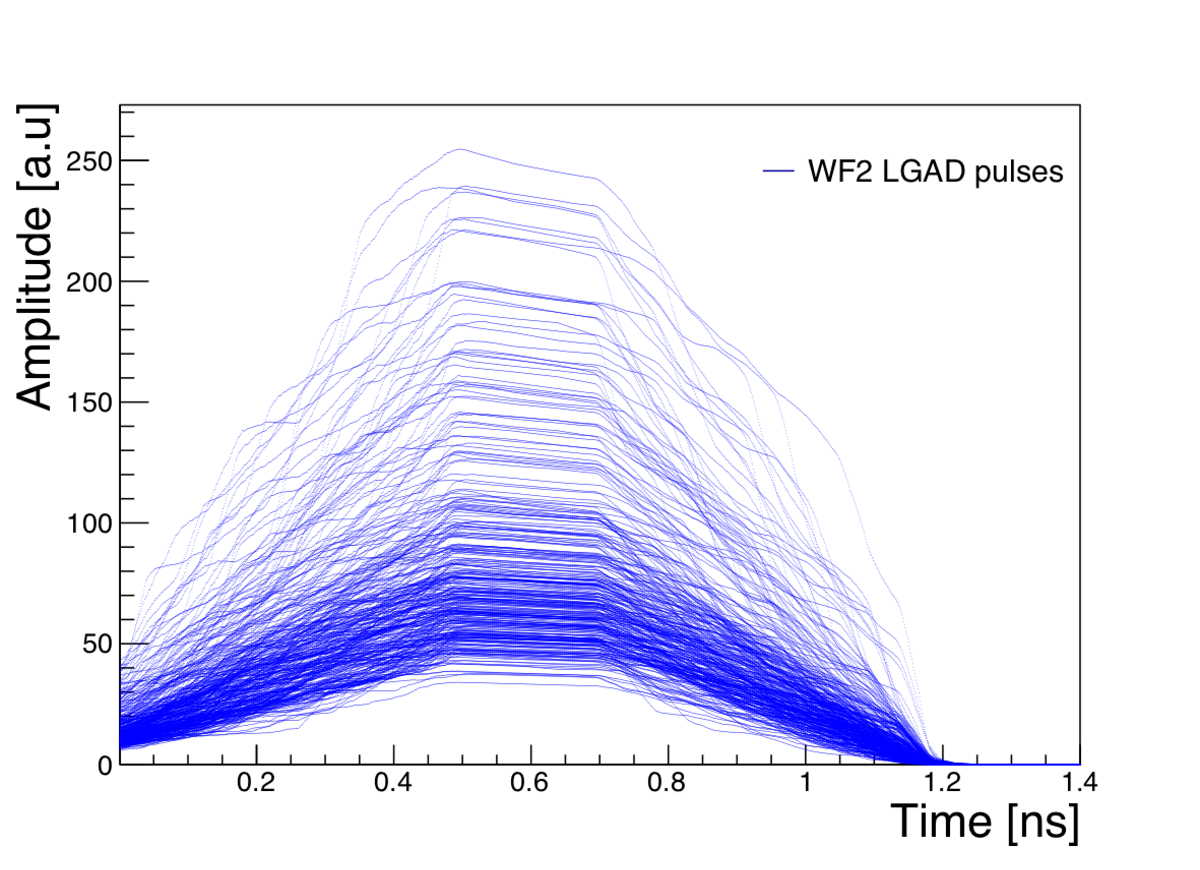
\includegraphics[width=0.48\textwidth]{figs/lgad_current_pre_rad_all_pulses_v3.pdf} \hfill
   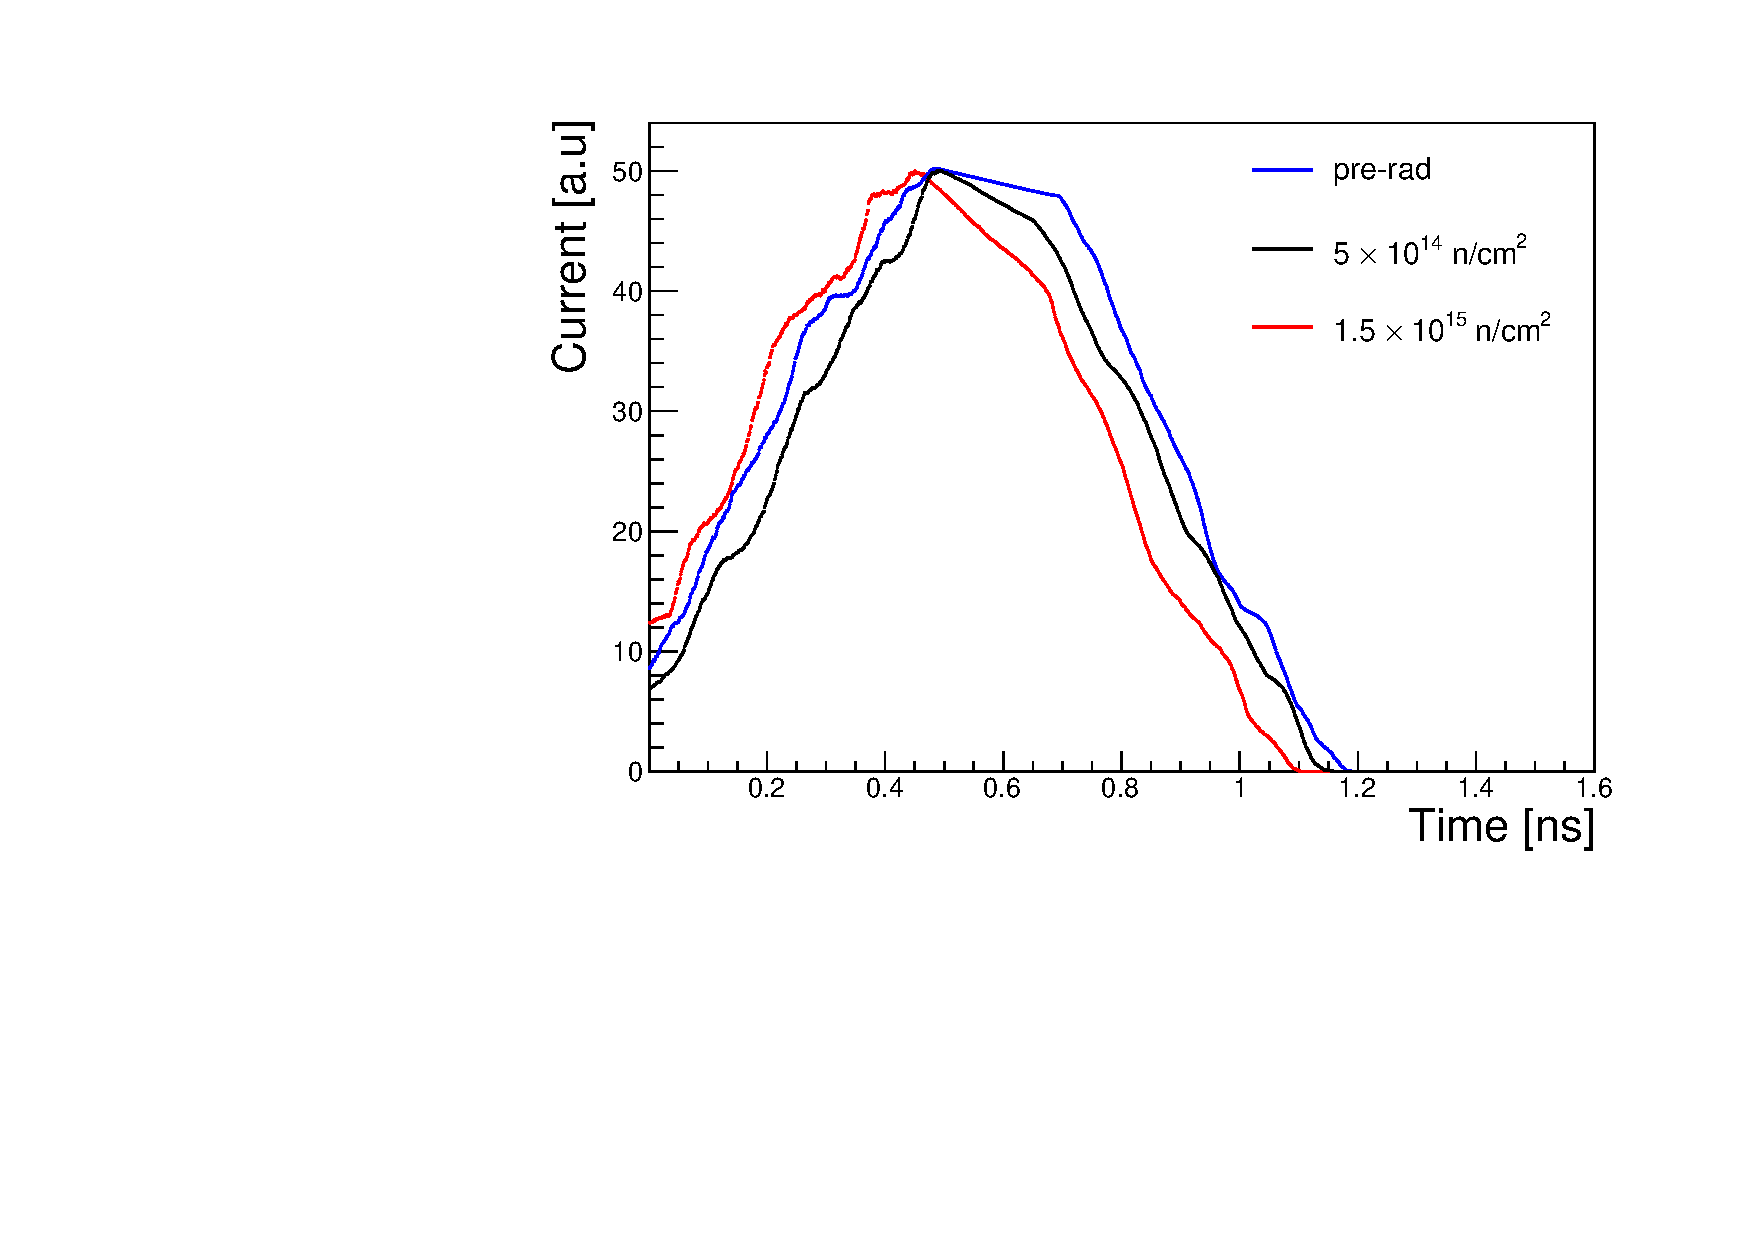
\includegraphics[width=0.48\textwidth]{figs/LGAD_current_all_irradiations_v2.pdf}
   \caption{(Left) One thousand simulated LGAD signal waveforms from WF2 for a pre-radiated sensor.
   (Right) Characteristic example LGAD signal waveforms for different irradiation levels.}
   \label{fig:lgad_current}
 \end{figure}


A waveform analysis is performed with the pulses obtained at the output of the
FEE block. We assign timestamps to each pulse by using algorithms that emulate
ideal LE and CF discriminators~\cite{Spieler}. For each threshold we obtain an LE and CF
timestamp as well as the corresponding time-over-theshold (ToT) of the pulse.
The ToT is defined as the time it takes between the first time the pulse crosses
the threshold and the second time the pulse crosses the threshold in the opposite direction. 
The SNR is defined as the ratio of the MPV of the amplitude distribution to the
r.m.s of the amplitude distribution of sampled noise-only waveforms.
On the left of Fig.~\ref{fig:amp_and_noise}, we show the amplitude distribution fitted to a Landau function, from
which the MPV is obtained, and on the right we show the noise distribution for a fixed sampling period for a 
pre-radiated sensor with SNR of 30. We scan over three different SNR scenarios: 20, 30, and 100, 
representing the cases corresponding to end-of-life sensors, new sensors, and new sensors
operated at very high gain. A schematic diagram of the
simulation is shown in Fig.~\ref{fig:simulation_diagram}.



\begin{figure}[htbp]
  \centering
  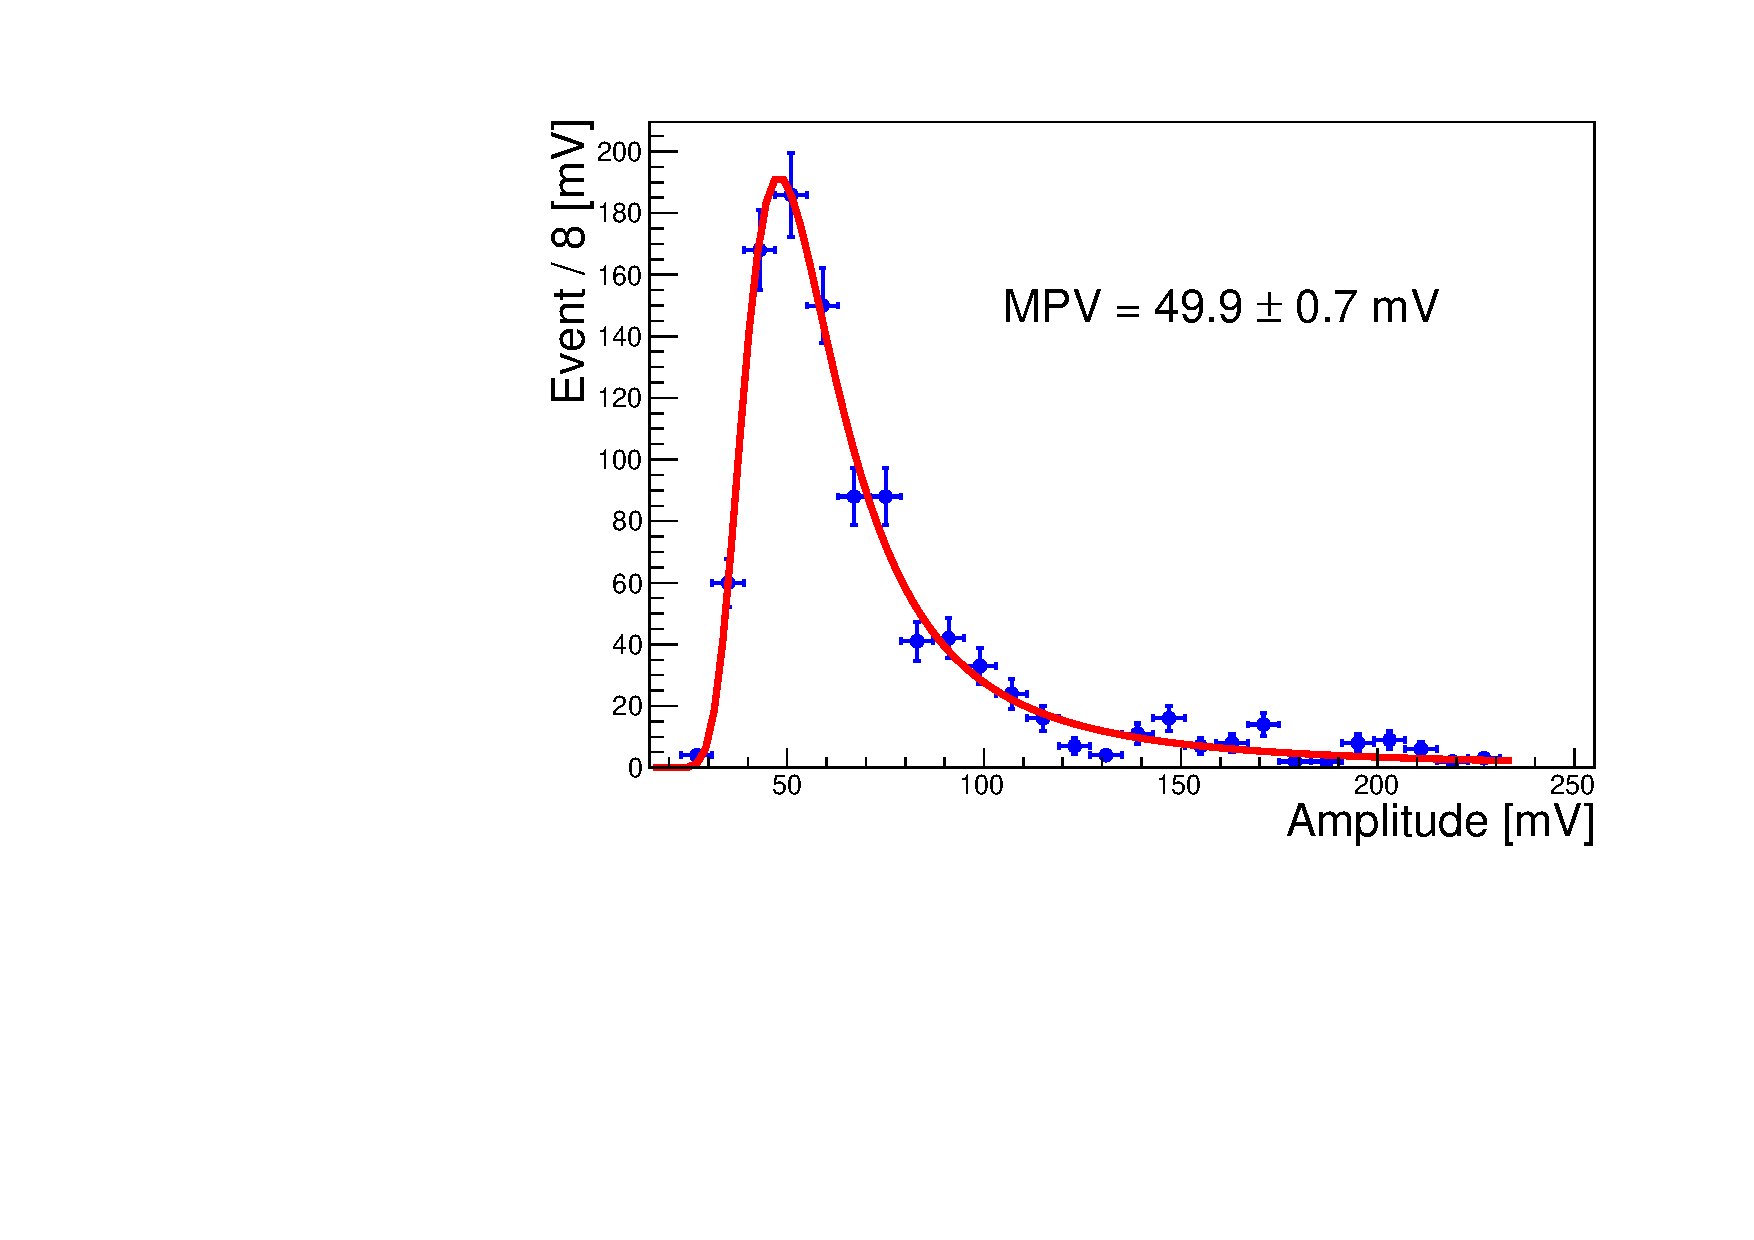
\includegraphics[width=0.48\textwidth]{figs/amplitude_1ns_landau_fit.pdf} \hfill
  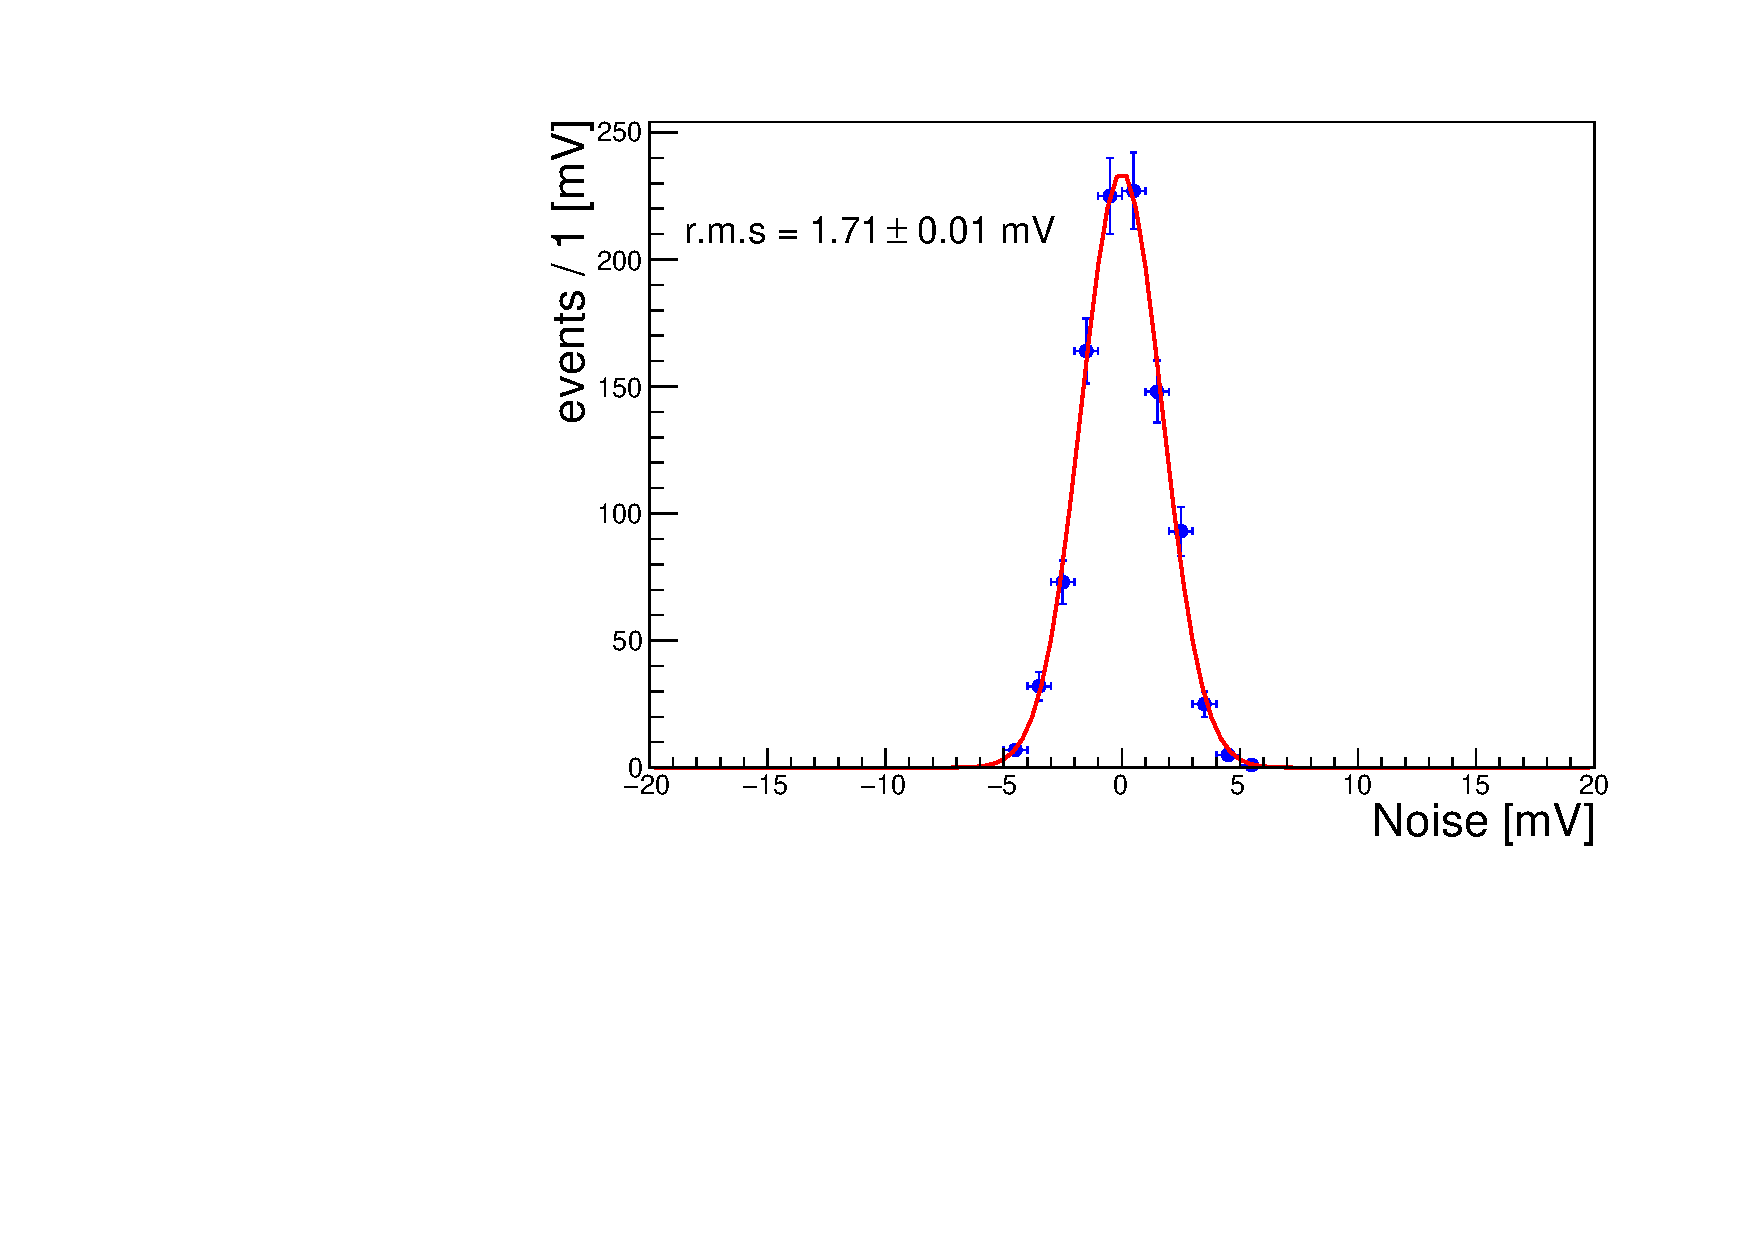
\includegraphics[width=0.48\textwidth]{figs/noise_plot_snr30.pdf}
  \caption{(Left) The amplitude distribution after the FEE. A Landau fit is performed to obtain the MPV.
  (Right) Amplitude distribution at a fixed sample of noise-only waveforms. A gaussian fit performed to obtain the r.m.s.
  Both figures correspond to a pre-radiation sensor using a shaping time of 1~\si{ns} and a SNR of 30.}
  \label{fig:amp_and_noise}
\end{figure}

\begin{figure}[htbp]
\centering
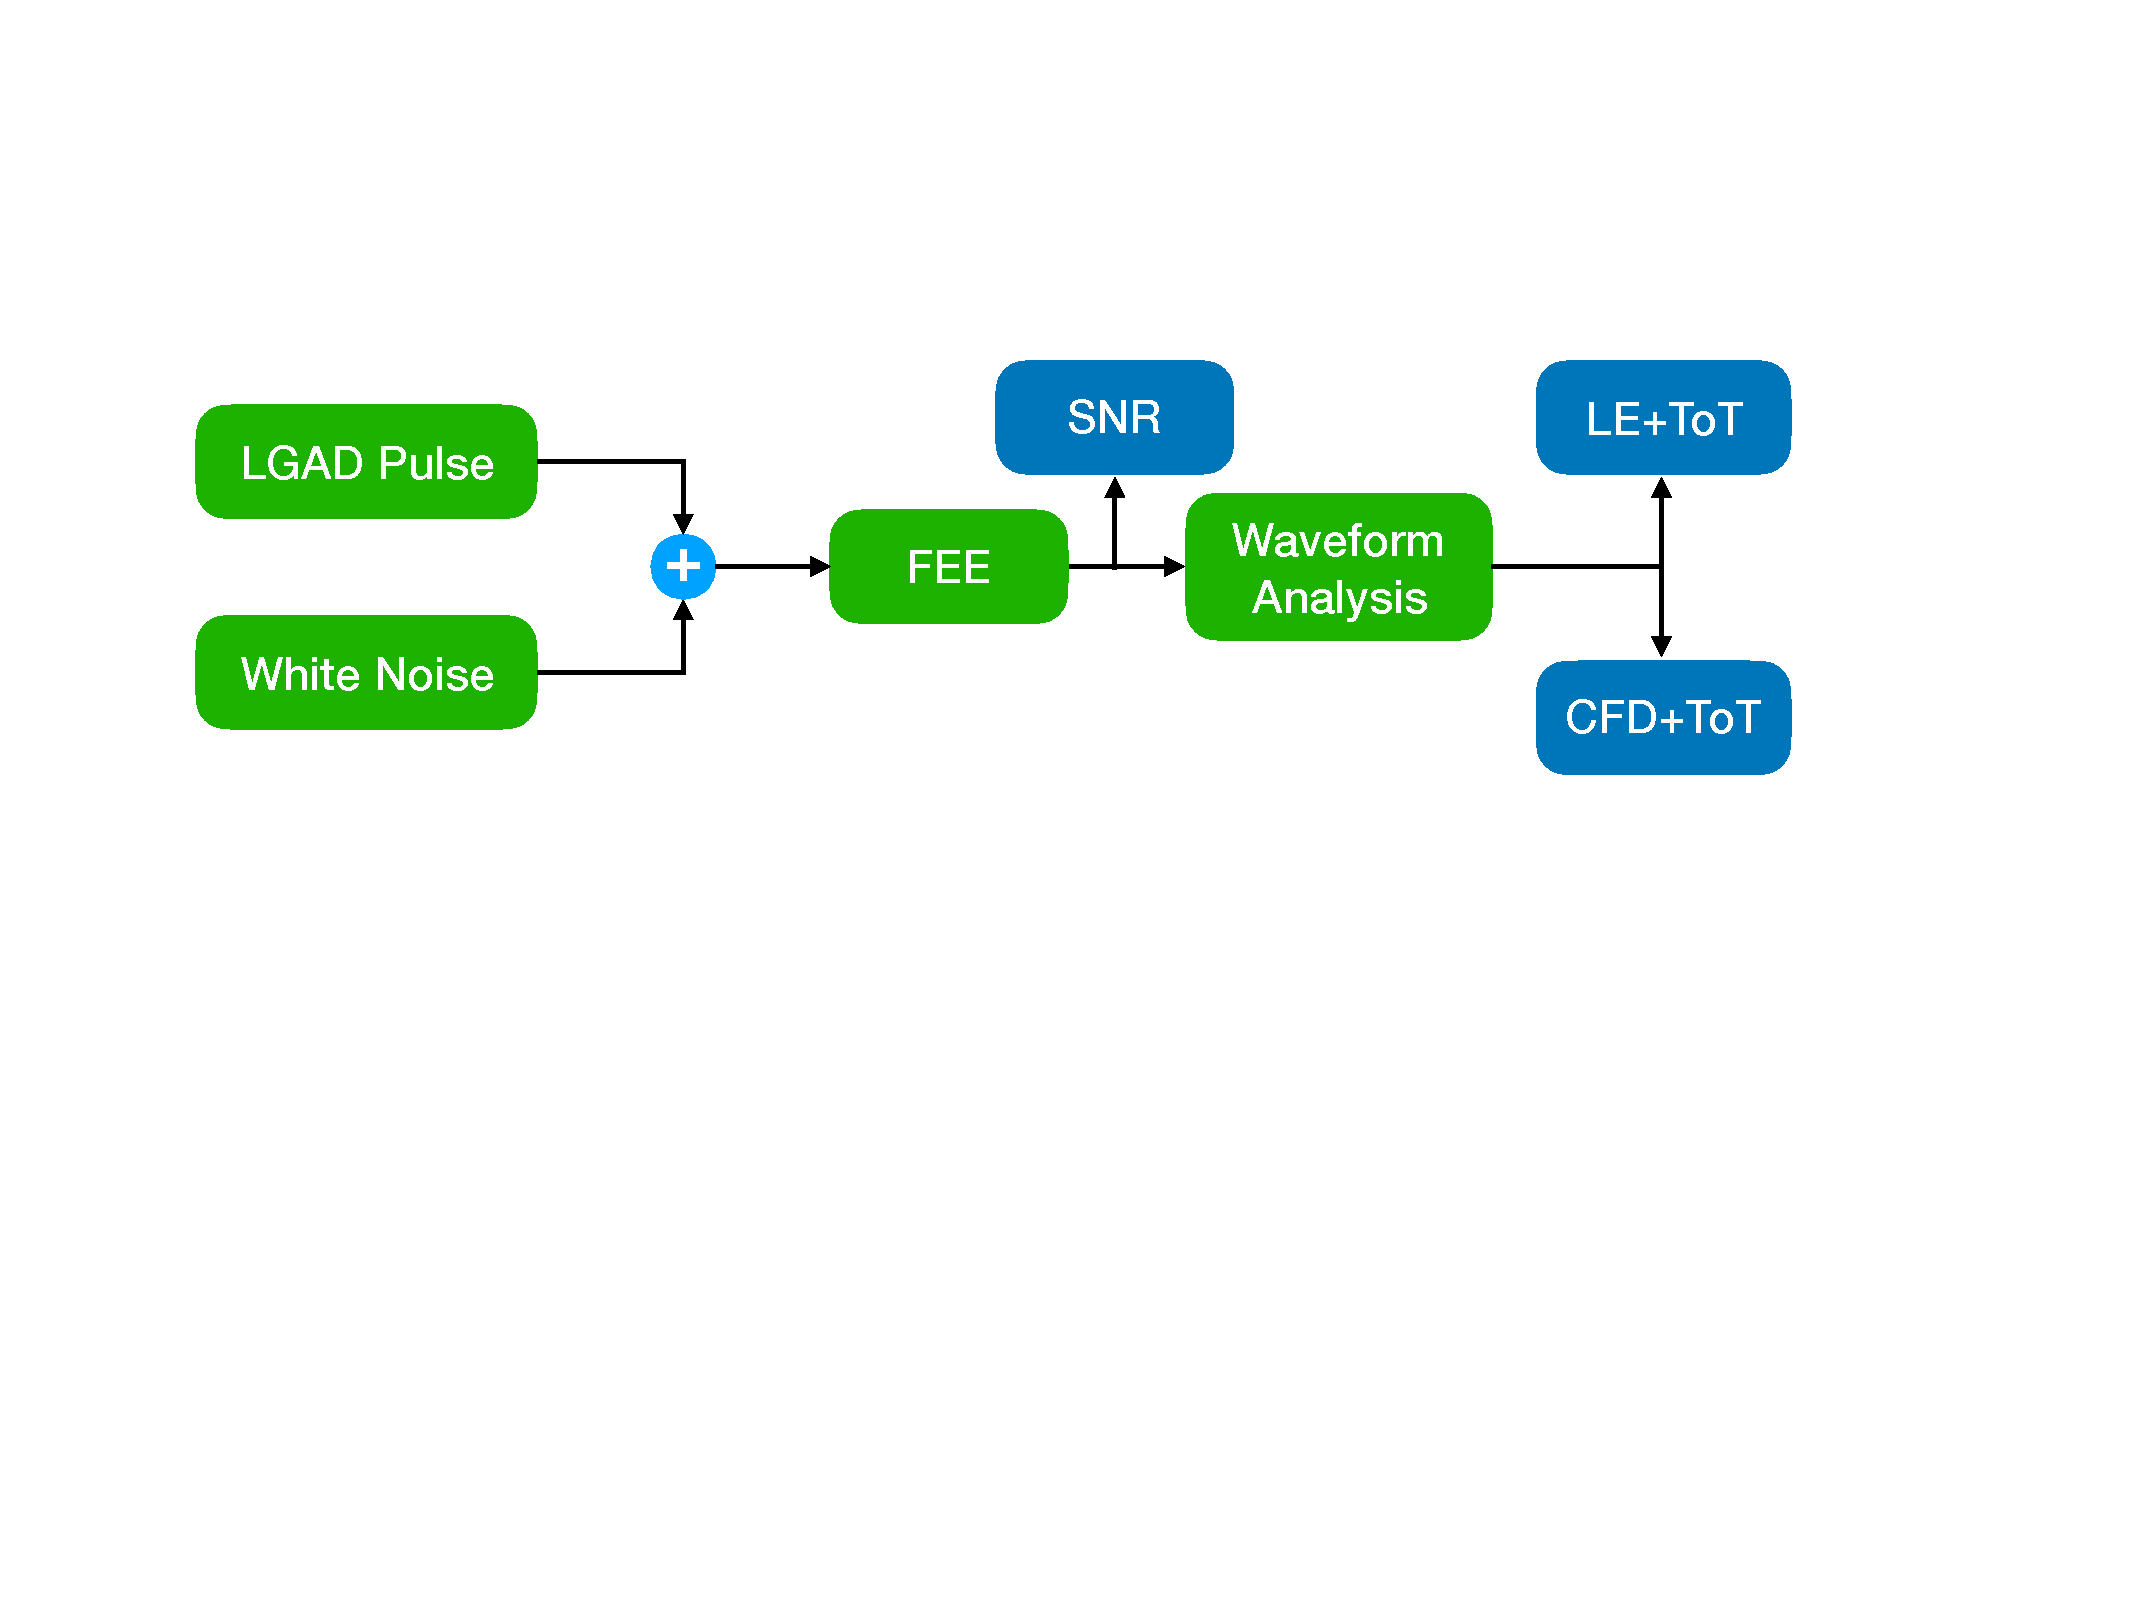
\includegraphics[width=0.75\textwidth]{figs/lgad_simulation_diagram.pdf}
\caption{A schematic diagram of the simulation. Each simulation configurable
	block is shown in green. The most relevant outputs of the simulation are shown
	in blue.} \label{fig:simulation_diagram}
\end{figure}



\subsection{Front-end electronics and noise injection}
\label{sub_sec:fee_simulation_and_noise} The front-end simulation combines
analytical and numerical calculations. We implement two independent
paths of simulations, one based on the time domain and the other on the Laplace domain.
Both simulation use the unprocessed WF2 LGAD pulses as input (see Fig~\ref{fig:lgad_current}).
The results of the two simulations are in agreement within statistical uncertainties and provide a
cross check of the results. Sections~\ref{sec:fee}
and~\ref{sec:noise_simulation} describe the details of the implementation of the
front-end and noise simulation. 

\subsubsection{Front-end simulation}\label{sec:fee}
The simulation of the front-end readout electronics is based on a single amplification stage. 
The FEE is a second order low-pass filter with transfer function ($H(S)$)
and impulse response ($h(t)$) given by equations~\ref{eq:filter_tf} and~\ref{eq:filter_ir}, respectively.
It realizes a $\mathrm{CR-RC}^{3}$-type filter~\cite{Sansen}.
 
 \begin{equation}\label{eq:filter_tf}
   H(S) = \frac{\frac{1}{\tau_{s}^{2}}}{(S+1/\tau_{s})^{2}}
 \end{equation}
 
 \begin{equation}\label{eq:filter_ir}
     h(t) = \frac{t}{\tau_s^2}e^{-t/\tau_{s}}
 \end{equation}
 
The output pulse of the FEE is the time domain convolution of the
unprocessed LGAD signal pulse from WF2 and the FEE impulse response function,
given in Eq.~\ref{eq:filter_ir}. The sampling period for the pulses and the
convolution is chosen to be 10~\si{ps} to maintain the needed numerical 
precision, and this choice is maintained throughout the simulation study. 
We focus our study on the BW of the FEE and to that
end we scan the $\tau_{s}$ parameter in Eq.~\ref{eq:filter_ir}, hereafter refered to as
the shaping time (ST),  through the following set:\{0.5, 1, 2, 4\}~\si{ns}. 
This set reflects the range of realistic FEE designs, given the power restrictions 
for the detector. Figure~\ref{fig:ir_and_lgad} (left) shows the comparison of the
impulse response and a characteristic example LGAD response for an ST of 1~\si{ns} while
Figure~\ref{fig:ir_and_lgad} (right) shows the LGAD response for all STs
studied. The LGAD response peaks later with respect to the
impulse response, and the slew rate is decreased in the first nanosecond
of the pulse. The pulse risetime, defined as the time required for the signal to rise from 10\% to 90\% of its
amplitude,  increases with the ST. Table~\ref{tab:risetime} summarizes the risetime
for the set of ST studied. 

\begin{figure}[htbp]
  \centering
  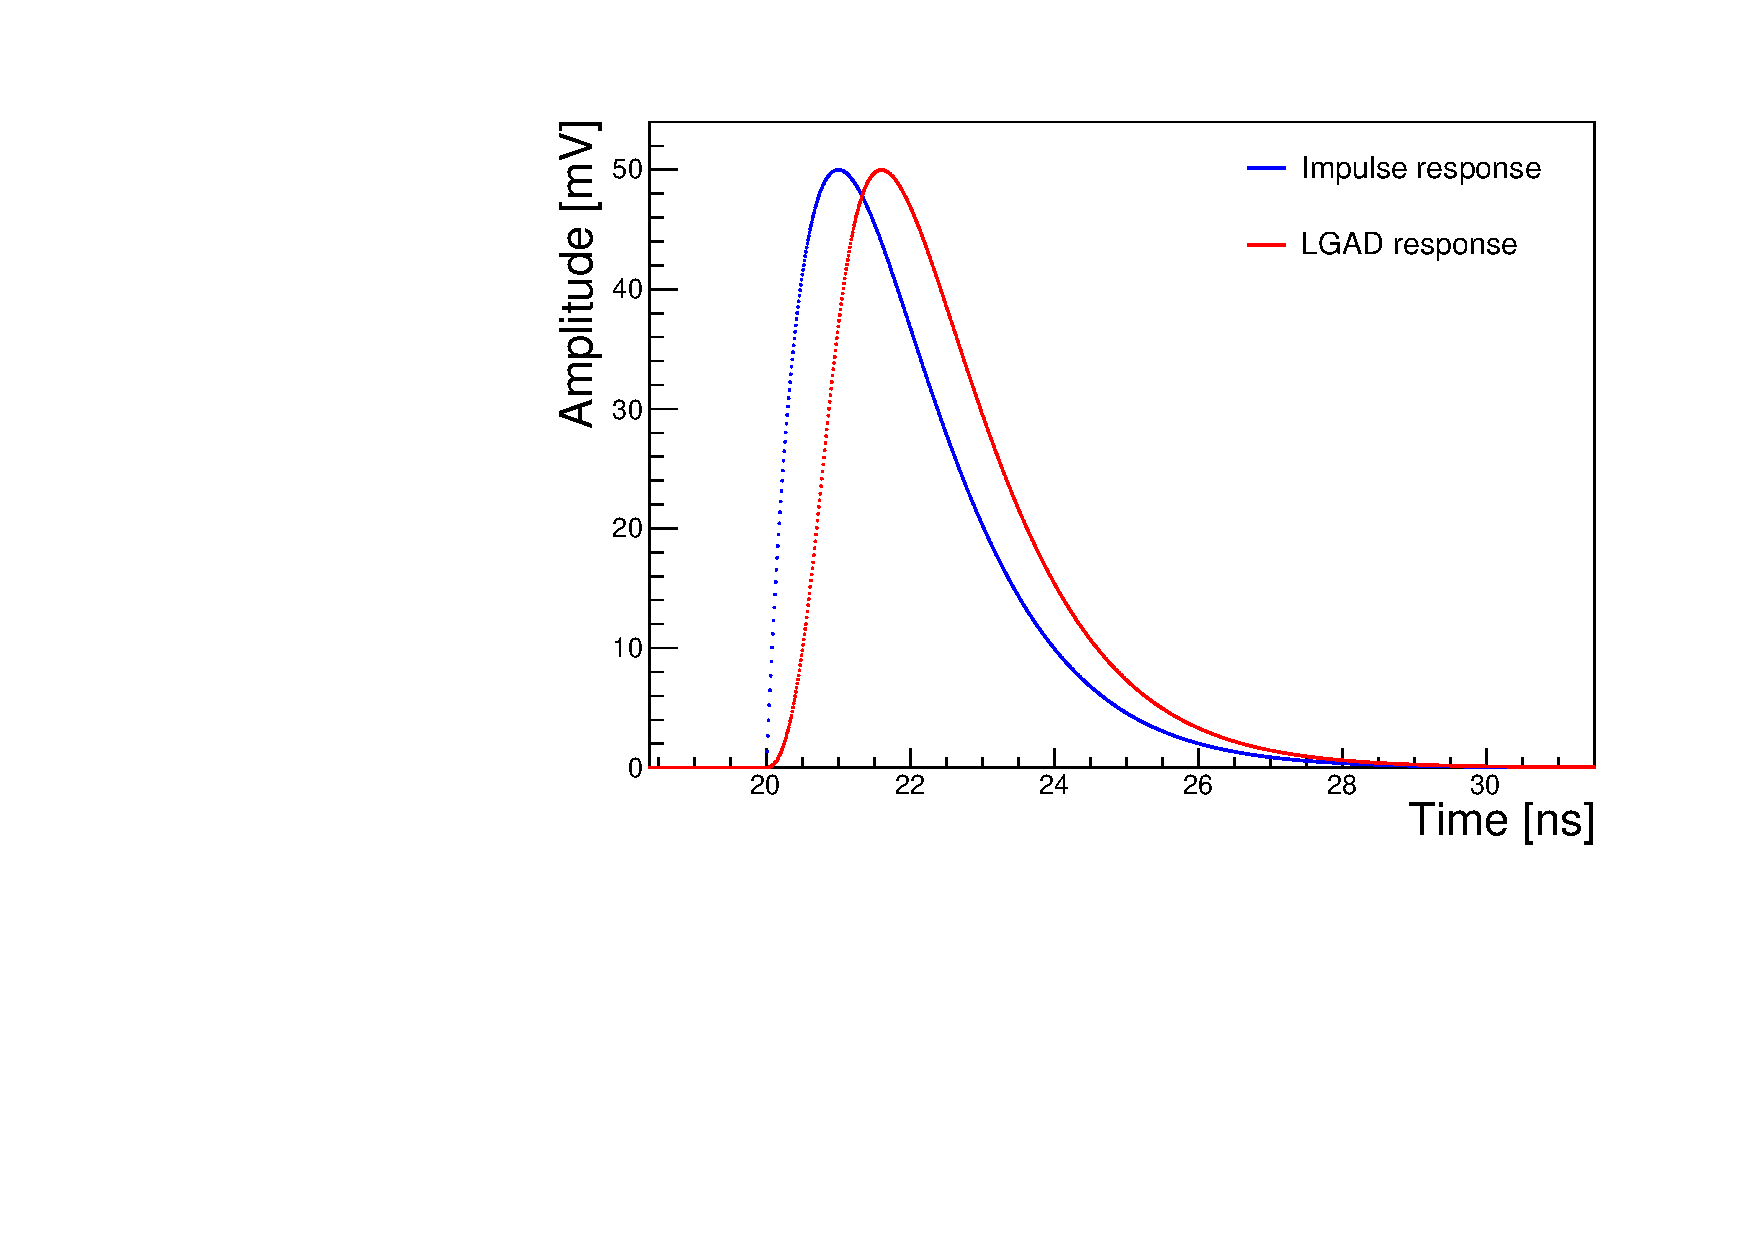
\includegraphics[width=0.48\textwidth]{figs/impulse_vs_lgad_response_1ns_shaping.pdf} \hfill
  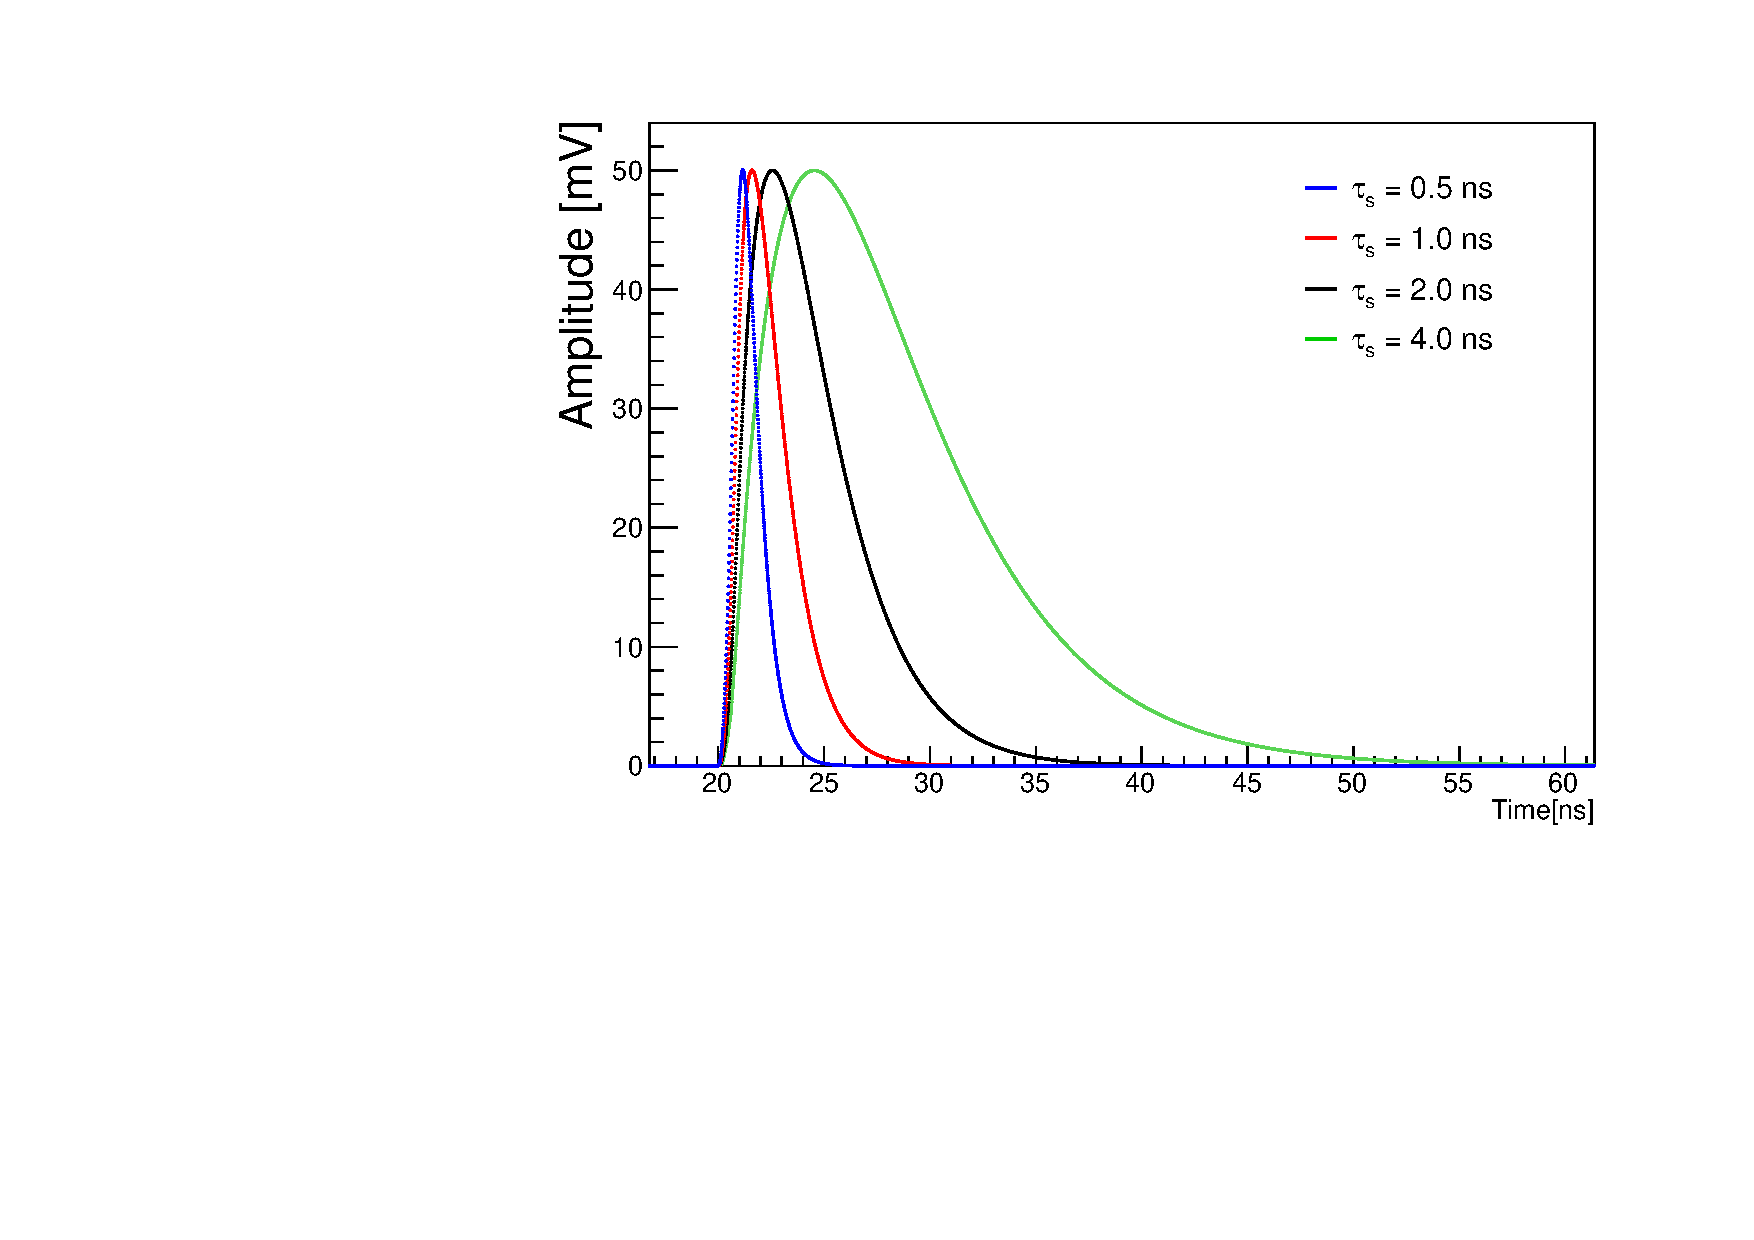
\includegraphics[width=0.48\textwidth]{figs/lgad_all_shaping_time_noiseless.pdf}
  \caption{(Left) Comparison of impulse and characteristic LGAD responses for the a shaping time (ST) of 1~\si{ns}.
  (Right) LGAD response for the four shaping times studied: \{0.5, 1, 2, 4\}~\si{ns}. All pulses have been normalized
  to achive a peak amplitude of 50~\si{mV}. }
  \label{fig:ir_and_lgad}
\end{figure}


\begin{table}
  \begin{center}
    \begin{tabular}{c|cccc}
    ST (ns) & 0.5  & 1.0 & 2.0 & 4.0 \\\hline
    Risetime (ns) & $0.7$ & $0.9$ & $1.4$ & $2.5$ \\
    \end{tabular}
    \caption{Measured risetime for all shaping times studied: \{0.5, 1, 2, 4\}~\si{ns}. The uncertainty is the r.m.s of the
    risetime distribution and is below 3\%.}
    \label{tab:risetime}
  \end{center}
 \end{table}


\subsubsection{Noise injection}\label{sec:noise_simulation}
Gaussian white noise is simulated by sampling every 10~\si{ps}~\cite{Radeka}. Each
sampled time is assigned a random amplitude which is drawn from a gaussian distribution with zero mean and width corresponding to the SNR under study. Based on Parseval's theorem, the noise amplitude needs to be adjusted depending
on the ST of the FEE for a given sampling rate. The left panel of Figure~\ref{fig:noise} shows the gaussian white 
noise before and after a filter with 1~\si{ns} shaping time. We checked that the average noise power spectrum is flat in the frequency domain up to at least 10 GHz. We observe the expected $\sqrt(\mathrm{BW})$ scaling of the noise after
the FEE for all the STs under study. The right panel of Figure~\ref{fig:noise} shows an example output of the
FEE block, with a 1~\si{ns} ST, for a pre-irradiated LGAD pulse after noise has been injected, with an SNR of 30. 

\begin{figure}[htbp]
  \centering
  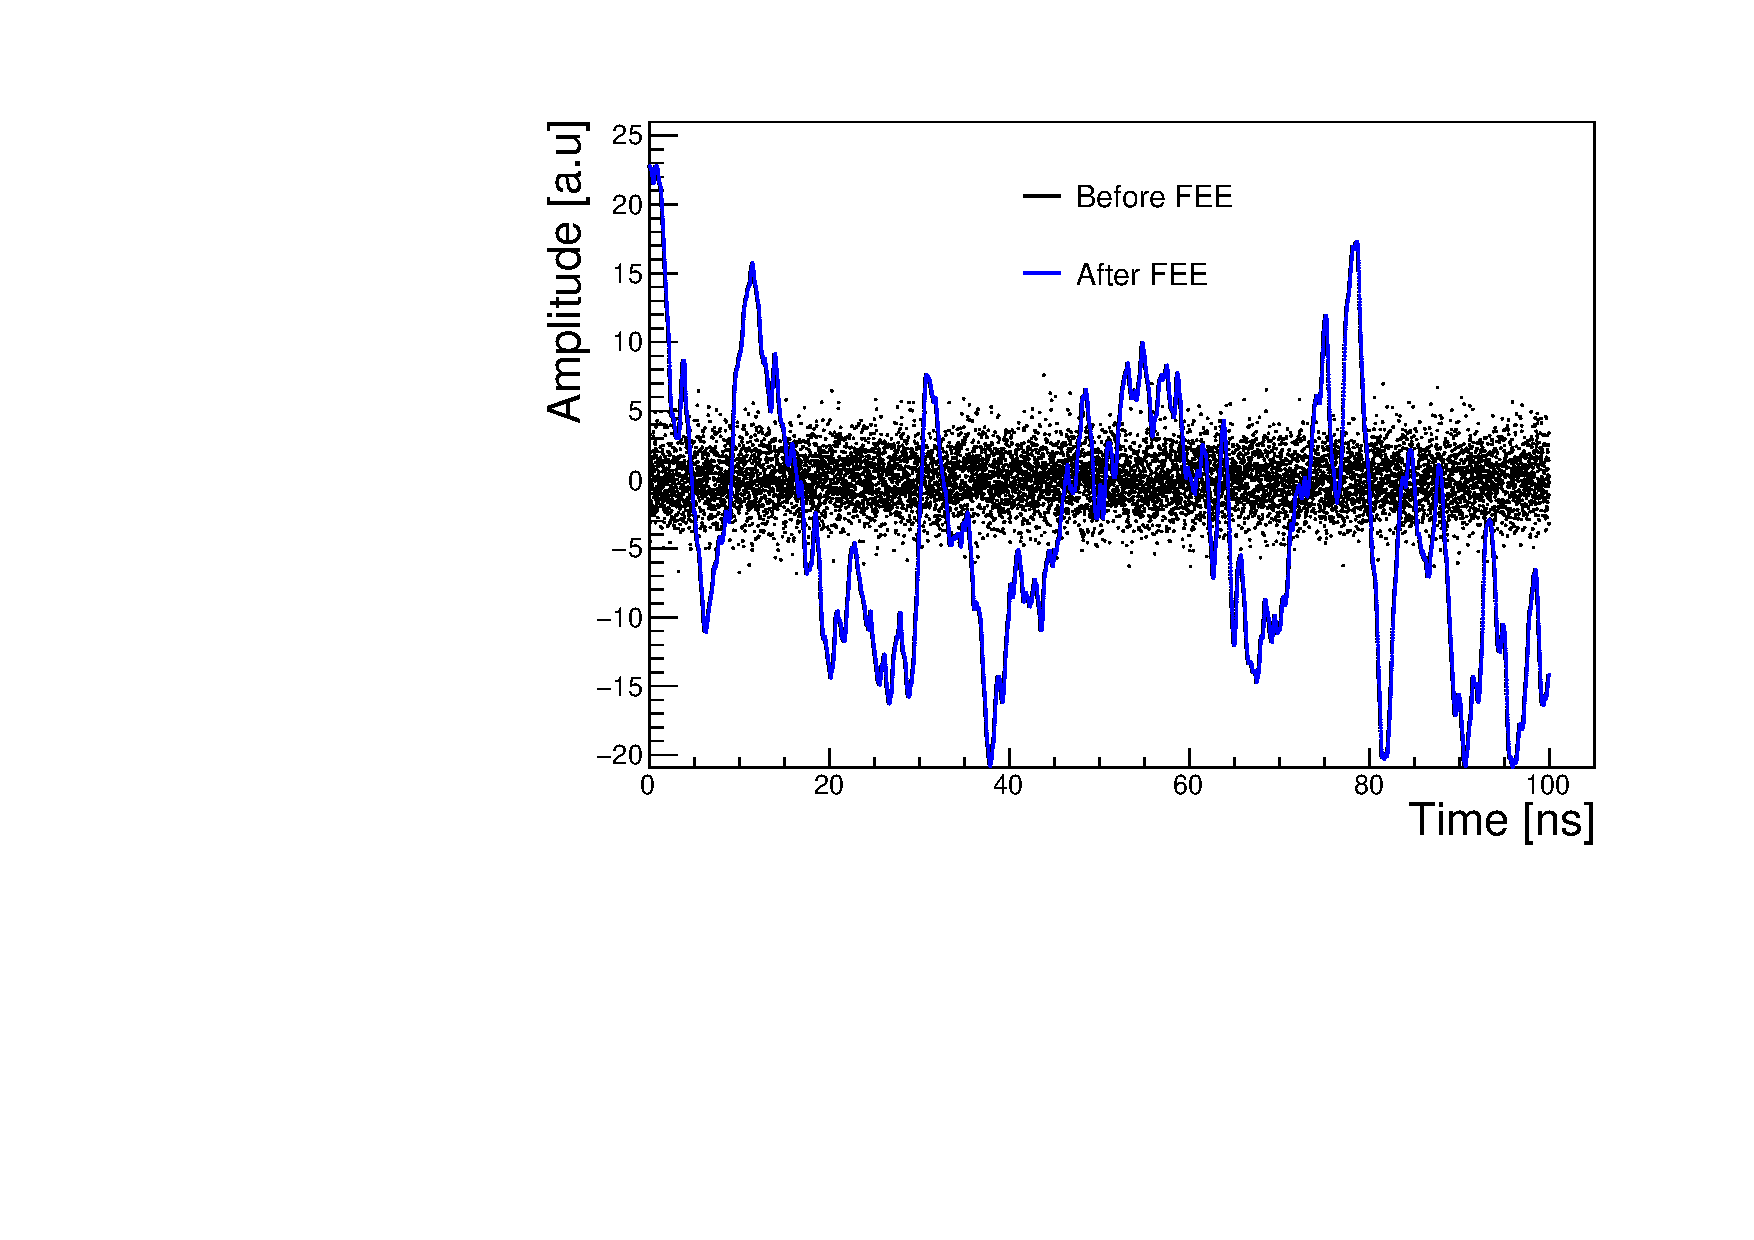
\includegraphics[width=0.48\textwidth]{figs/noise_vs_shaped_noise.pdf} \hfill
  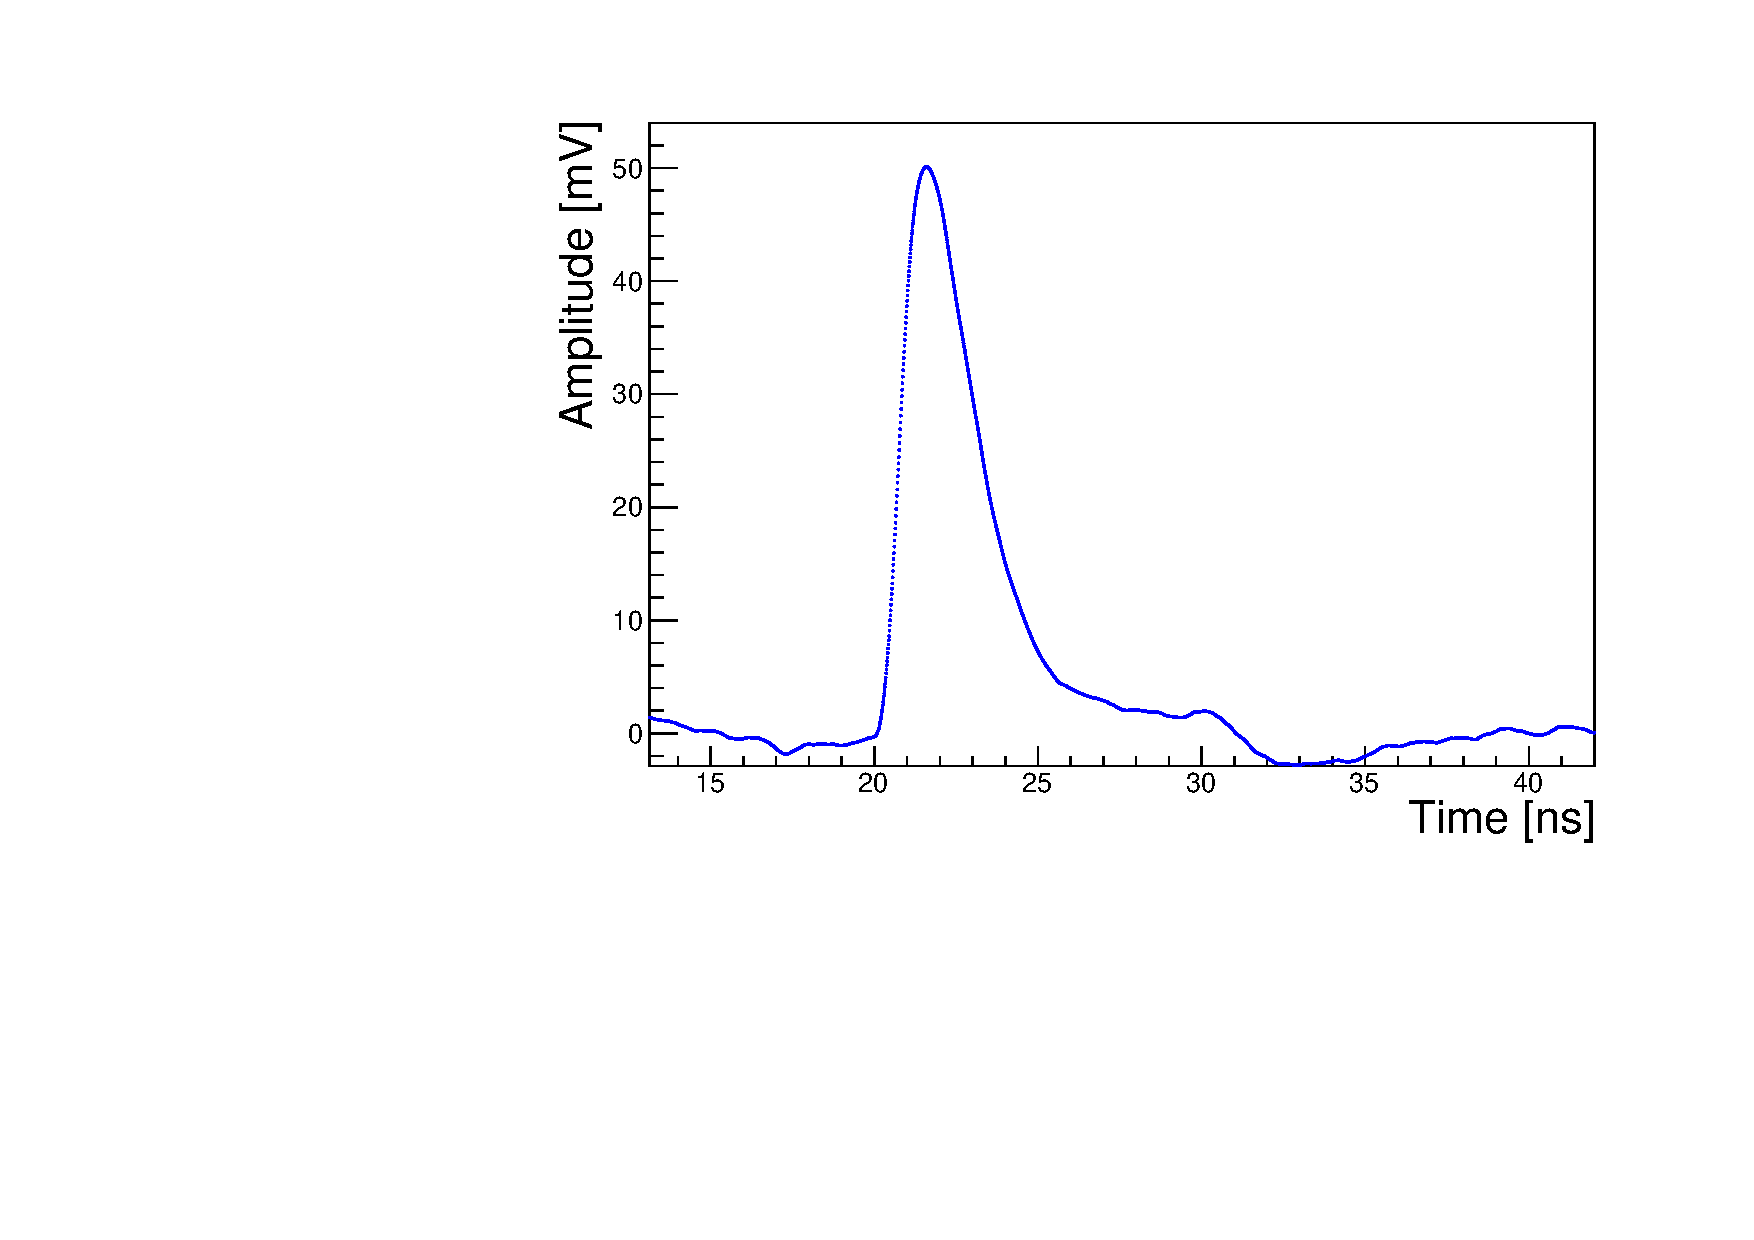
\includegraphics[width=0.48\textwidth]{figs/lgad_pre_rad_st_1ns_snr_30.pdf}
  \caption{(Left) Comparison of gaussian white noise before and after the FEE.
  (Right) Example pulse at the output of the FEE block with an SNR of 30. Both figures use a shaping time (ST) of 1~\si{ns}.}
  \label{fig:noise}
\end{figure}

\section{Timing reconstruction and analysis}\label{sec:timing_and_analysis}
The time reconstruction is based on waveform analysis. For each of the 1000 simulated LGAD waveforms, 
we generate the processed pulse by injecting the white noise and construct the processed waveform 
sampled every 10 ps. We assign a timestamp by determining when a given voltage threshold has been crossed. 
The threshold can be a constant value (LE) or a constant fraction of the pulse height (CF).
In the CF case, we also simulated two practical implementations based on subtracting
a scaled version of the original waveform from a delayed version. The delay is achieved either using an ideal 
delay element or an RC-type low pass filter. We observe that the practical CF timestamp implemented 
using an ideal delay element yields equivalent results as the ideal CF timestamp to within uncertainties. 
The more realistic CFD implemented using an RC-type low pass filter yields a slightly degraded performance.
We scan the LE and CF threshold such that we find the one with the best time resolution.
The timestamps are measured with a set of fixed bins of width 20~\si{ps} while the ToT is measured with fixed bins of width 100~\si{ps} binning in order to simulate the effect of time bin quantization. Scanning over the ToT bin size, we observed that the effect of ToT quantization was negligible for a resolution better than 200 ps.
The time resolution is estimated as the r.m.s of the timestamp distribution obtained for a particular threshold. 

  \begin{figure}[htbp]
    \centering
    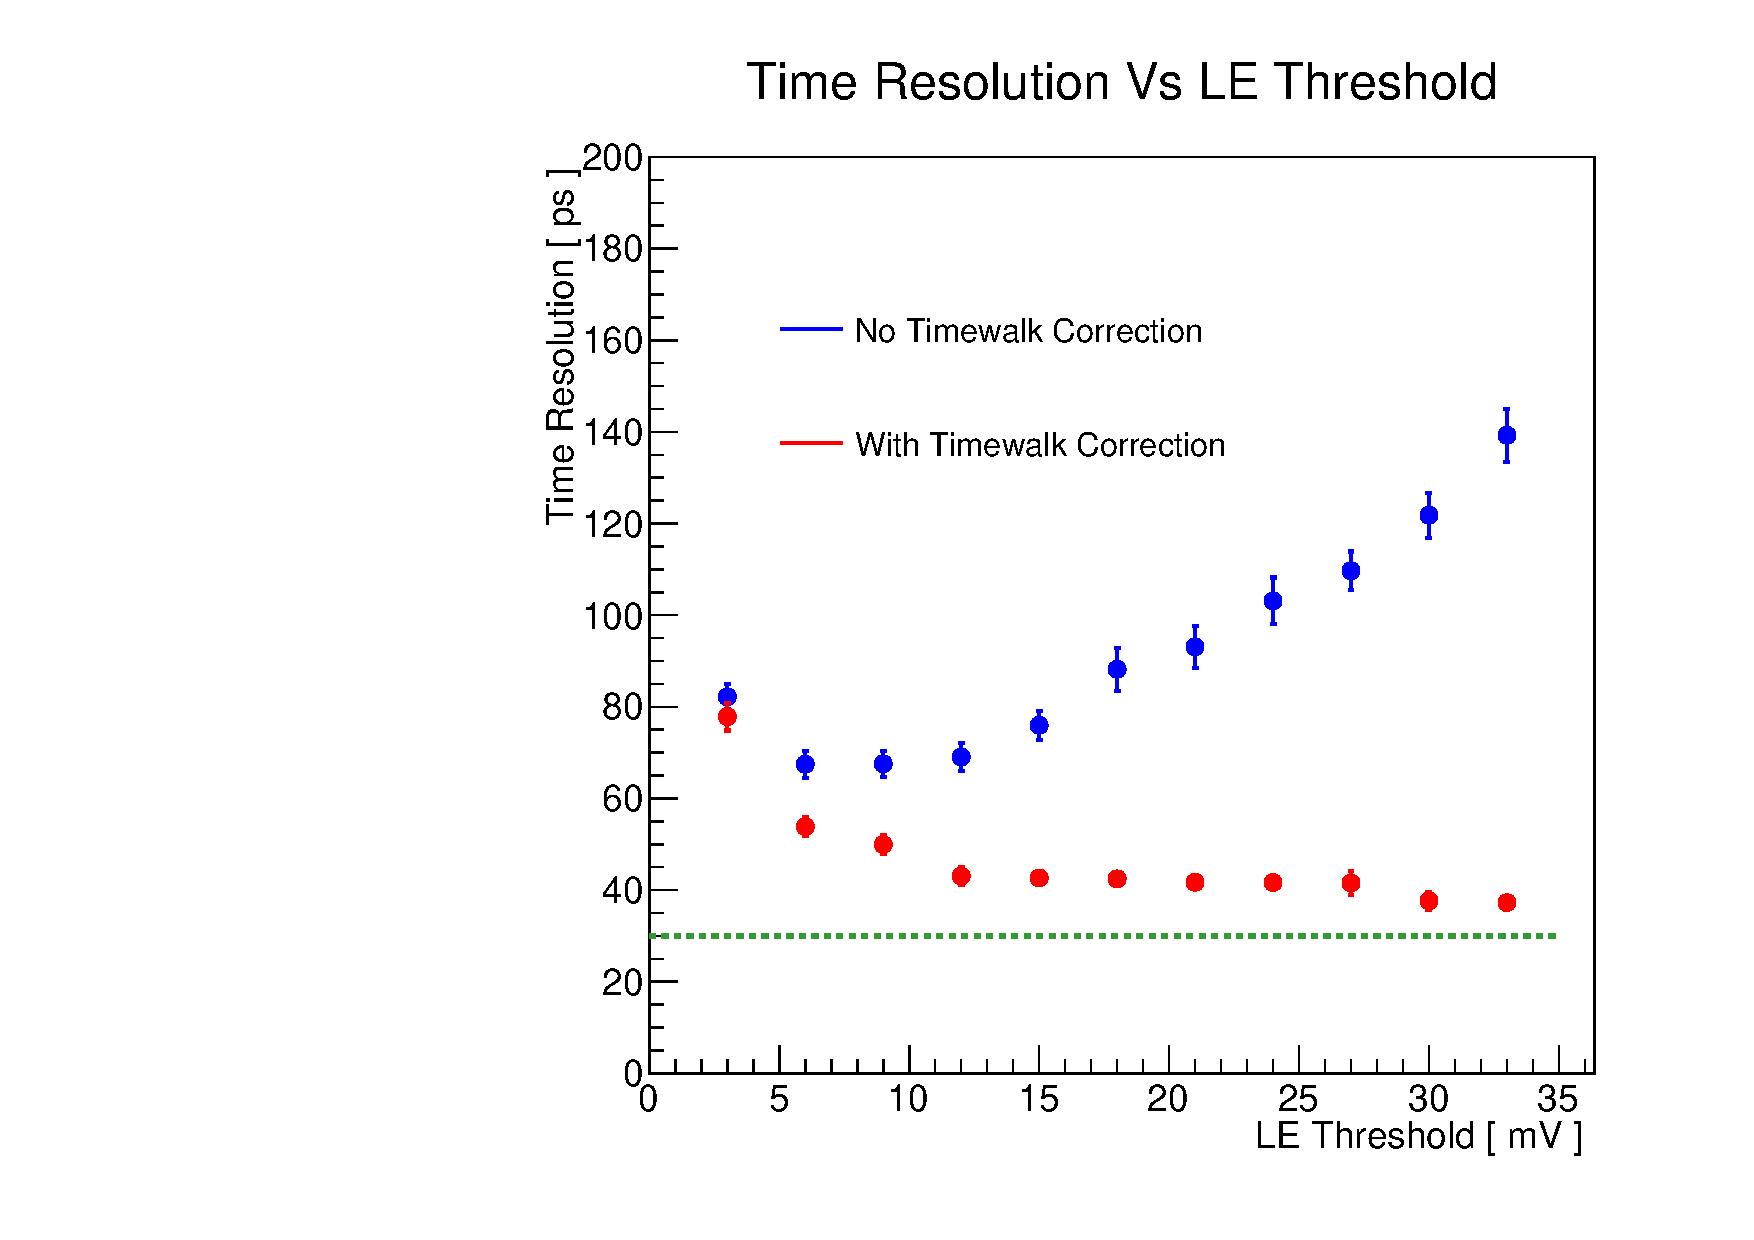
\includegraphics[width=0.48\textwidth]{figs/ShapingTime1p0_SNR30_55MicronGain15Prerad_FIXED_NOISE_FIXED_SNR_V2_converted_TimeResolutionVsThresholdToT.pdf} \hfill
    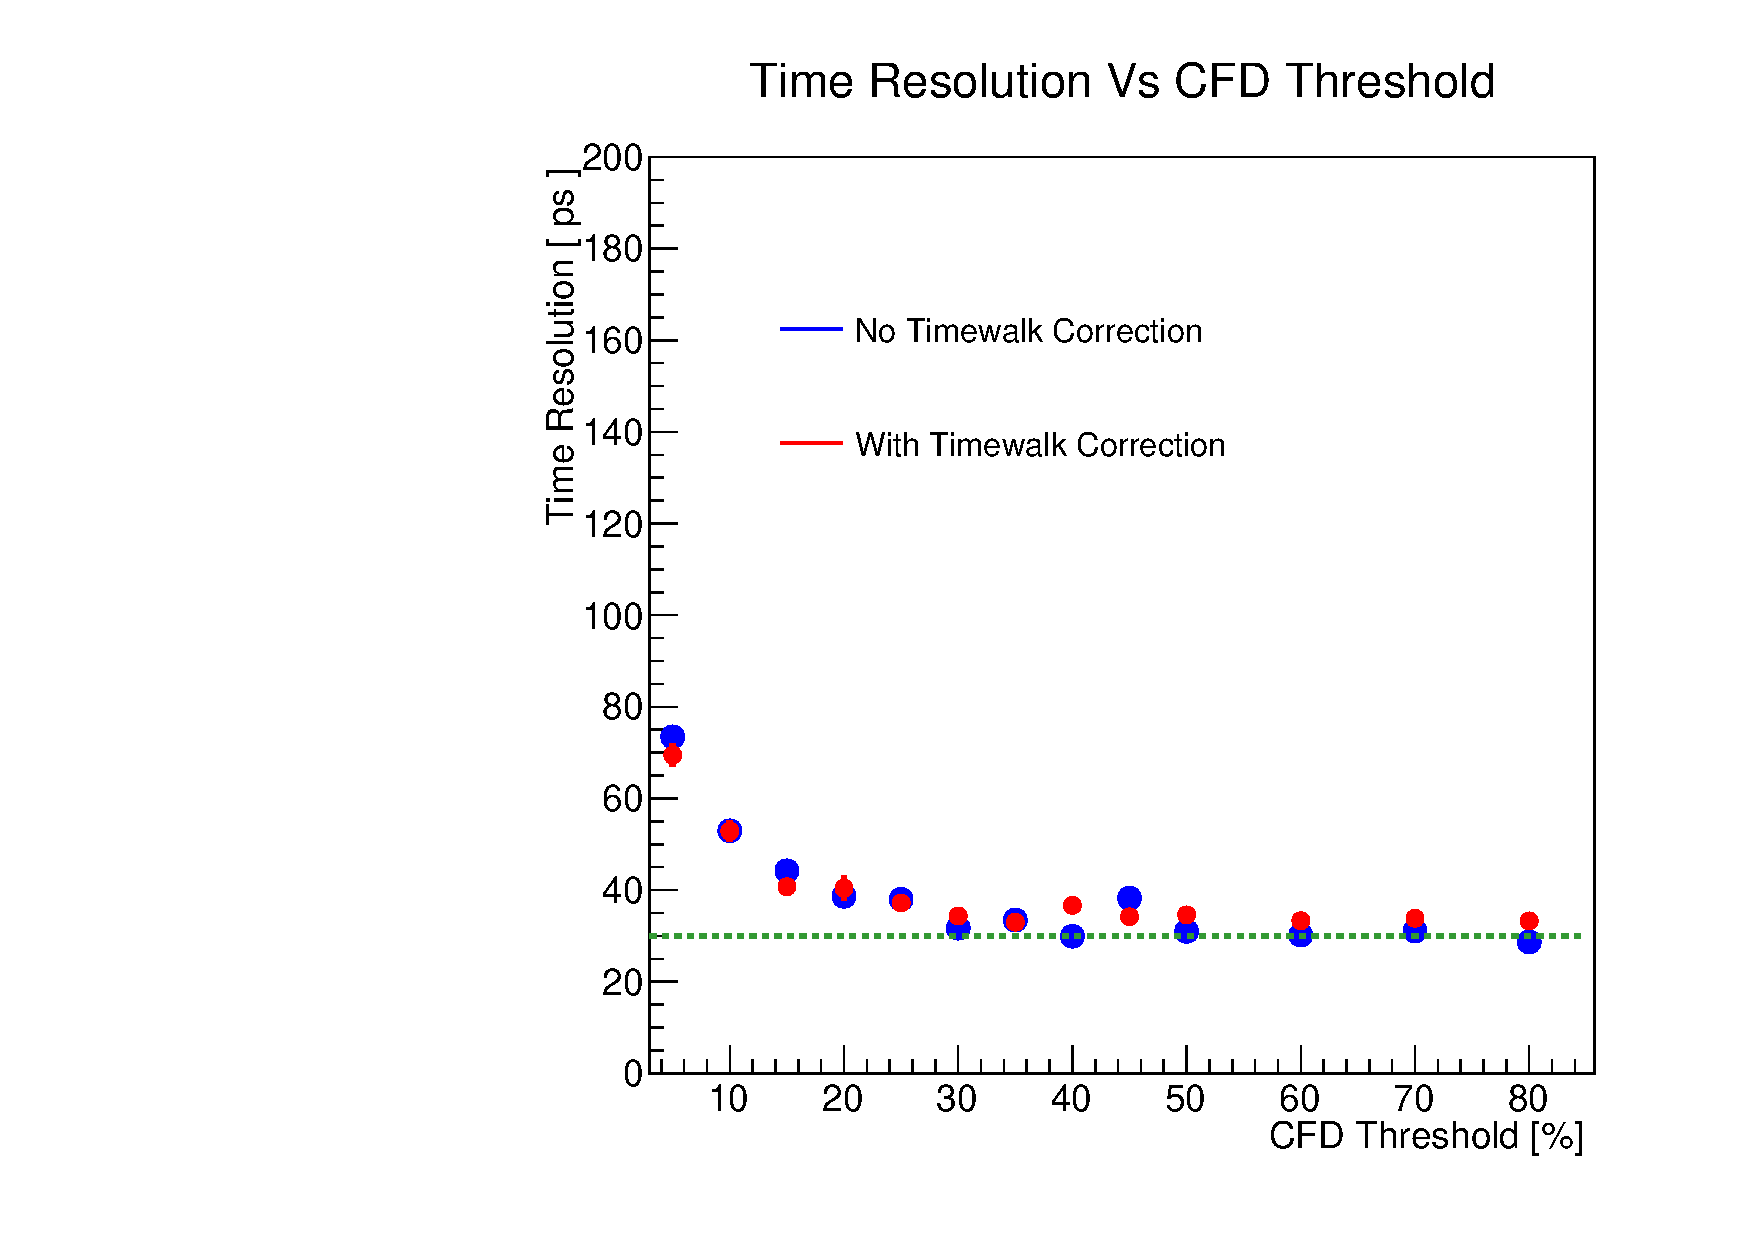
\includegraphics[width=0.48\textwidth]{figs/ShapingTime1p0_SNR30_55MicronGain15Prerad_FIXED_NOISE_FIXED_SNR_V2_converted_TimeResolutionVsThresholdCFD.pdf}
    \caption{(Left) LE time resolution as a function of threshold.
    (Right) CF time resolution as a function of threshold.
    Both figure use pre-irradiated LGAD sensor with a ST of 1 ns and a SNR of 30.}
    \label{fig:time_resolution_scan}
  \end{figure}

Figure~\ref{fig:time_resolution_scan} shows the time resolution as a function
of the threshold required for a pre-irradiated LGAD sensor with an ST of 1~\si{ns} and an SNR of 30.
We apply a time-walk correction aimed at correcting for the known effect of time drift as a function
of the pulse height, and ensuring that the time response is flat as a function of the pulse height. 
Figure~\ref{fig:ToT} (left) shows a typical two dimensional map of $t_{0}$ and ToT for the
LE algorithm, where a clear correlation between $t_{0}$ and ToT is observed. 
We construct a profile graph of $t_{0}$ versus ToT by calculating the mean $t_{0}$ in
each bin of ToT as shown on the right of Figure~\ref{fig:ToT}. We fit the profile graph to a 2nd-order polynomial to 
obtain the time-walk correction. The resulting analytical expression after the fit is then used to 
alleviate the dependence of $t_{0}$ on ToT. Different corrections are derived for each simulation scenario
characterized by the values of the simulation parameters: ST, SNR, and LGAD irradiation level.
As can be seen in Fig.~\ref{fig:time_resolution_scan}, the size of the time-walk correction 
depends on the threshold used, and applying the correction yields a large 
improvement on the time resolution measured using the LE algorithm. By construction, 
timestamps measured using the CF algorithm is largely insensitive to the time-walk effect.

\begin{figure}[htbp]
  \centering
  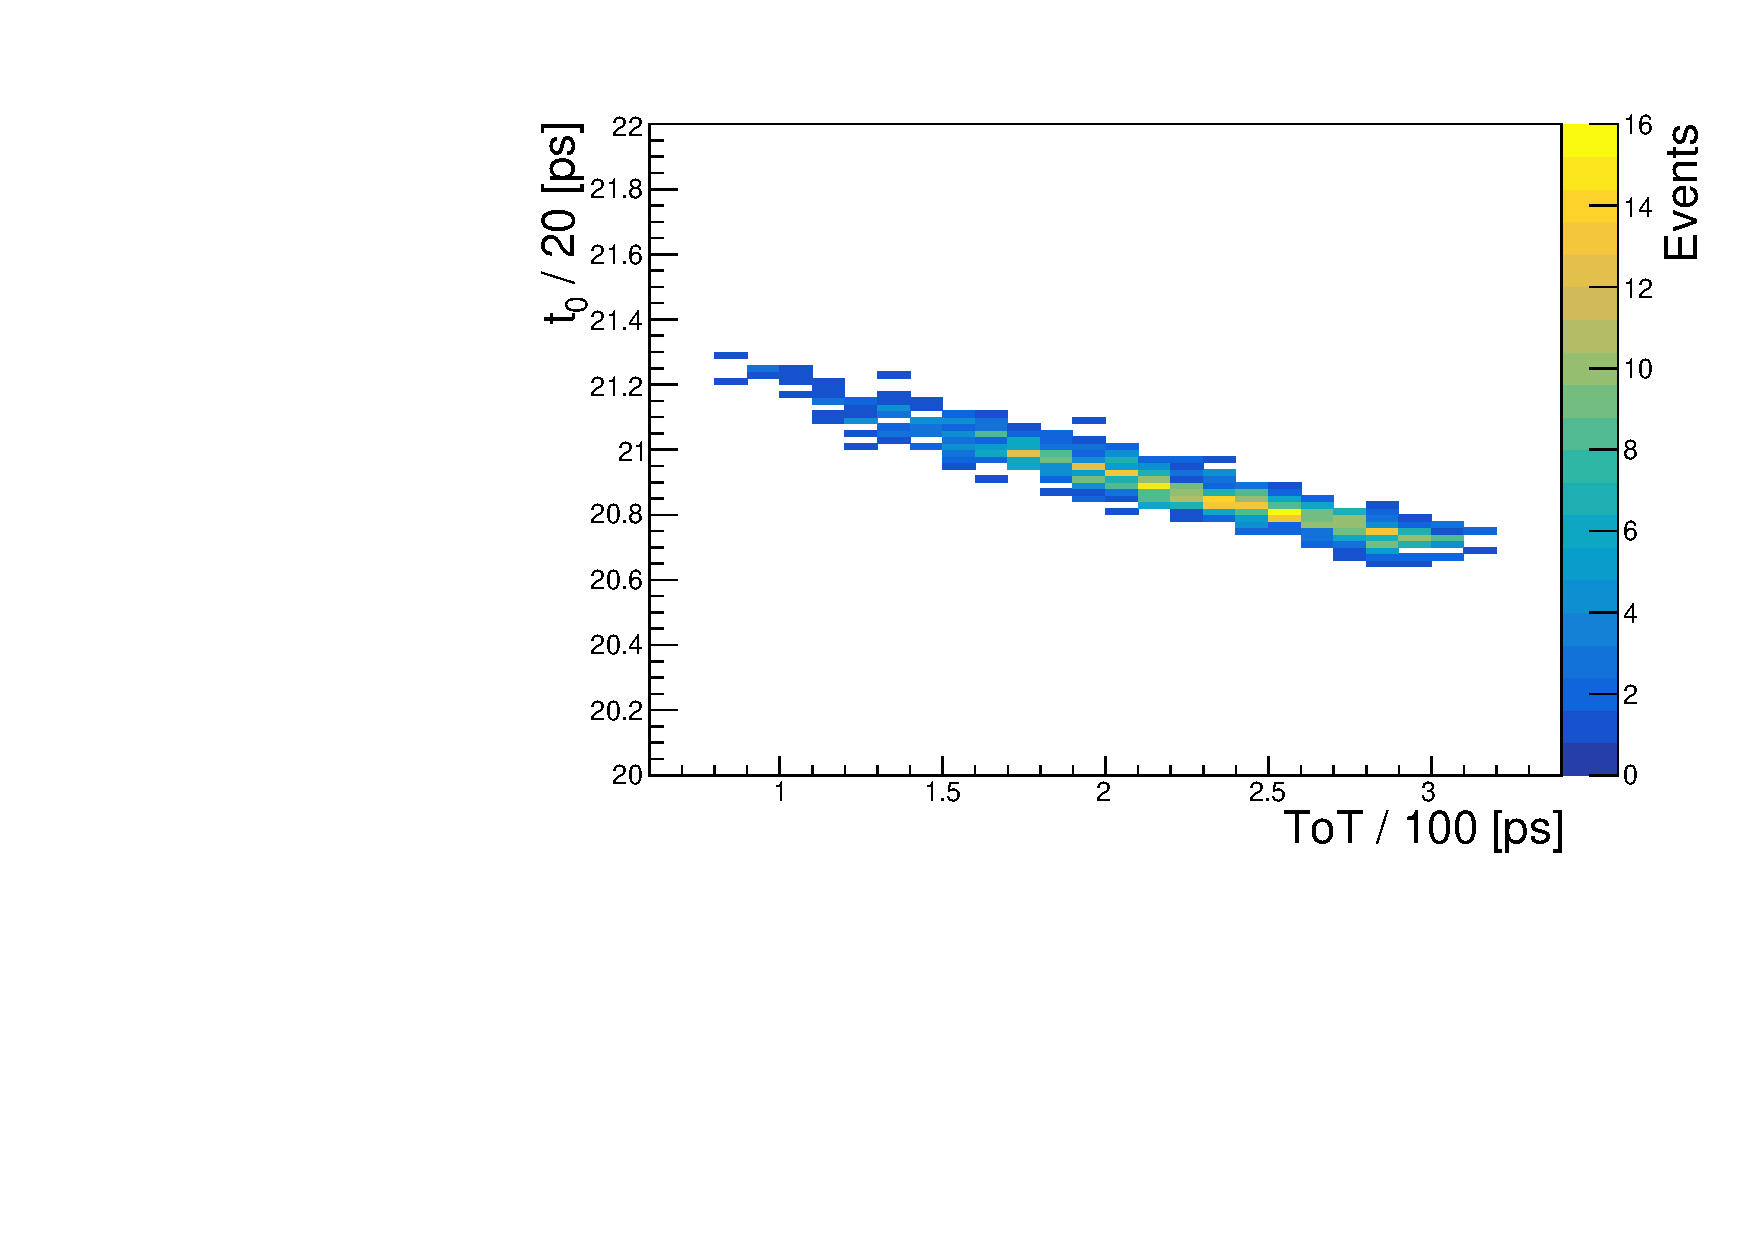
\includegraphics[width=0.48\textwidth]{figs/twoD_ToT_pre_rad_st_1ns_snr_30_le_tot_threshold_30mV_v2.pdf} \hfill
  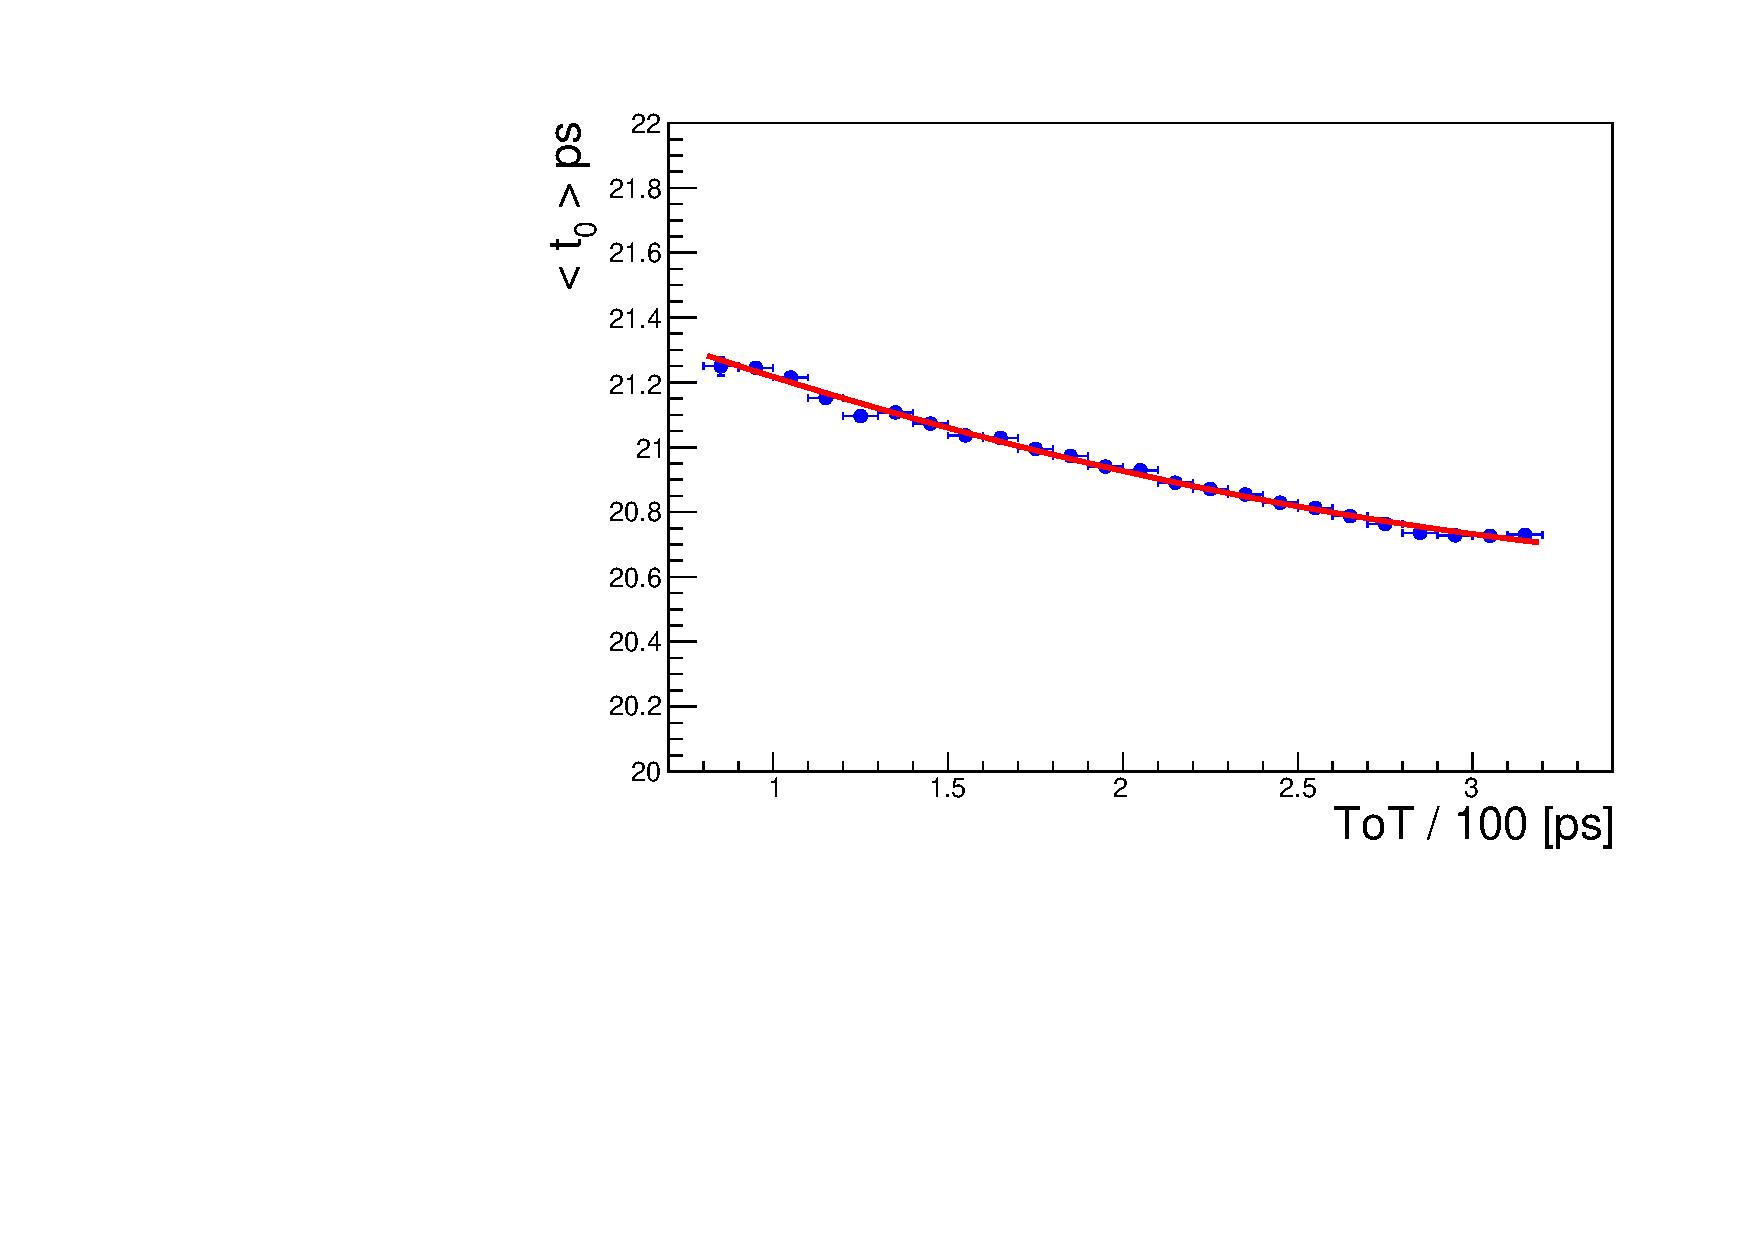
\includegraphics[width=0.48\textwidth]{figs/oneD_ToT_pre_rad_st_1ns_snr_30_le_tot_threshold_30mV_v2.pdf}
  \caption{(Left) two dimenasional map of the timestamp ($t_{0}$) and ToT ($t_{1} - t_{0}$).
  (Right) one dimensional projection of the timestamp ($t_{0}$) dependence on ToT, the red curve is the 2nd-order polinomial fit that
  ultimately is used to correct $t_{0}$. Both figures use a shaping time (ST) of 1~\si{ns} and correspond to a SNR of 30.}
  \label{fig:ToT}
\end{figure}


Fig.~\ref{fig:time_res} shows a typical $t_{0}$ distribution, using the LE and CF algorithms, for the pre-irradiated
LGAD sensor after the ToT correction has been applied. The time resolution ($\sigma_{t}$) is measured to be $37.3 \pm 1.4 $
and $33.0 \pm 1.4$ for the LE and CF, respectively. 

  \begin{figure}[htbp]
    \centering
    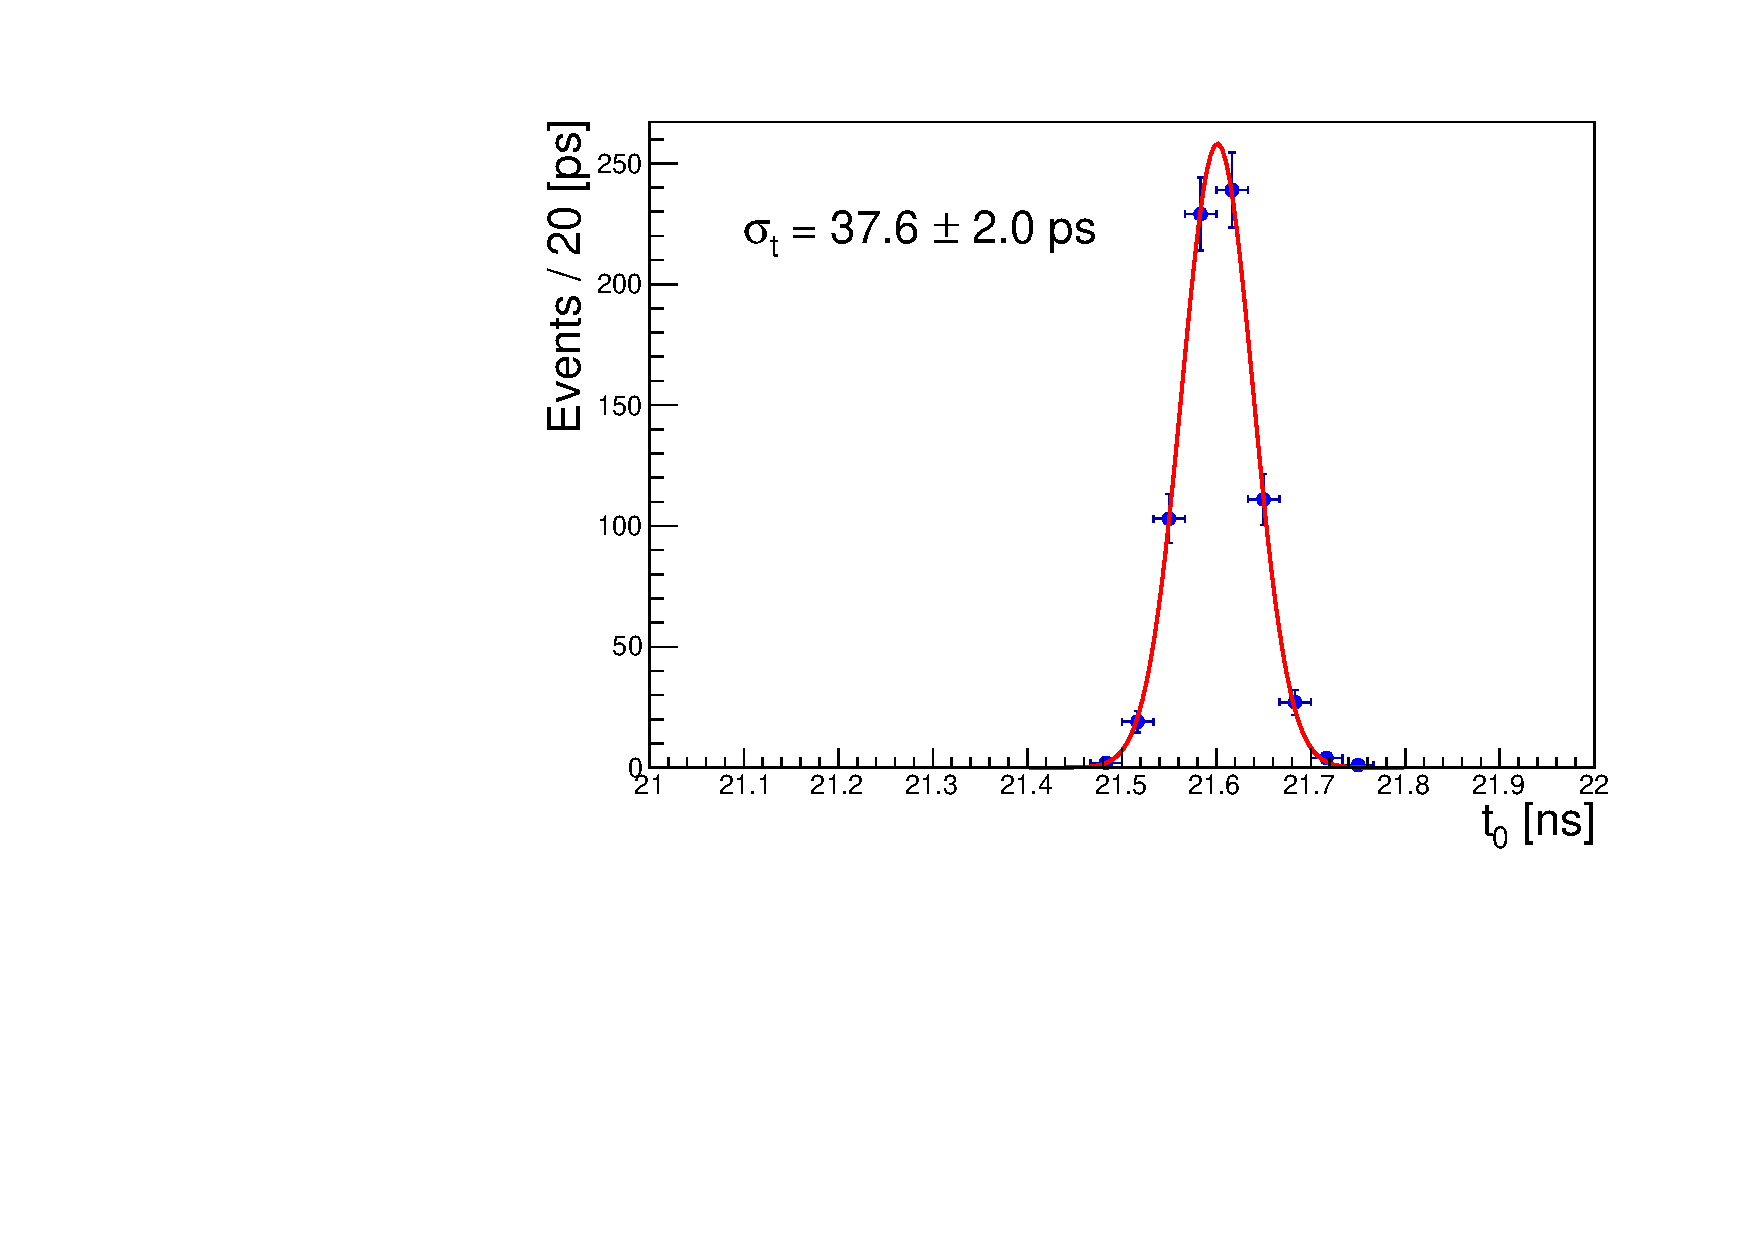
\includegraphics[width=0.48\textwidth]{figs/pre_rad_st_1ns_snr_30_le_tot_threshold_30mV.pdf} \hfill
    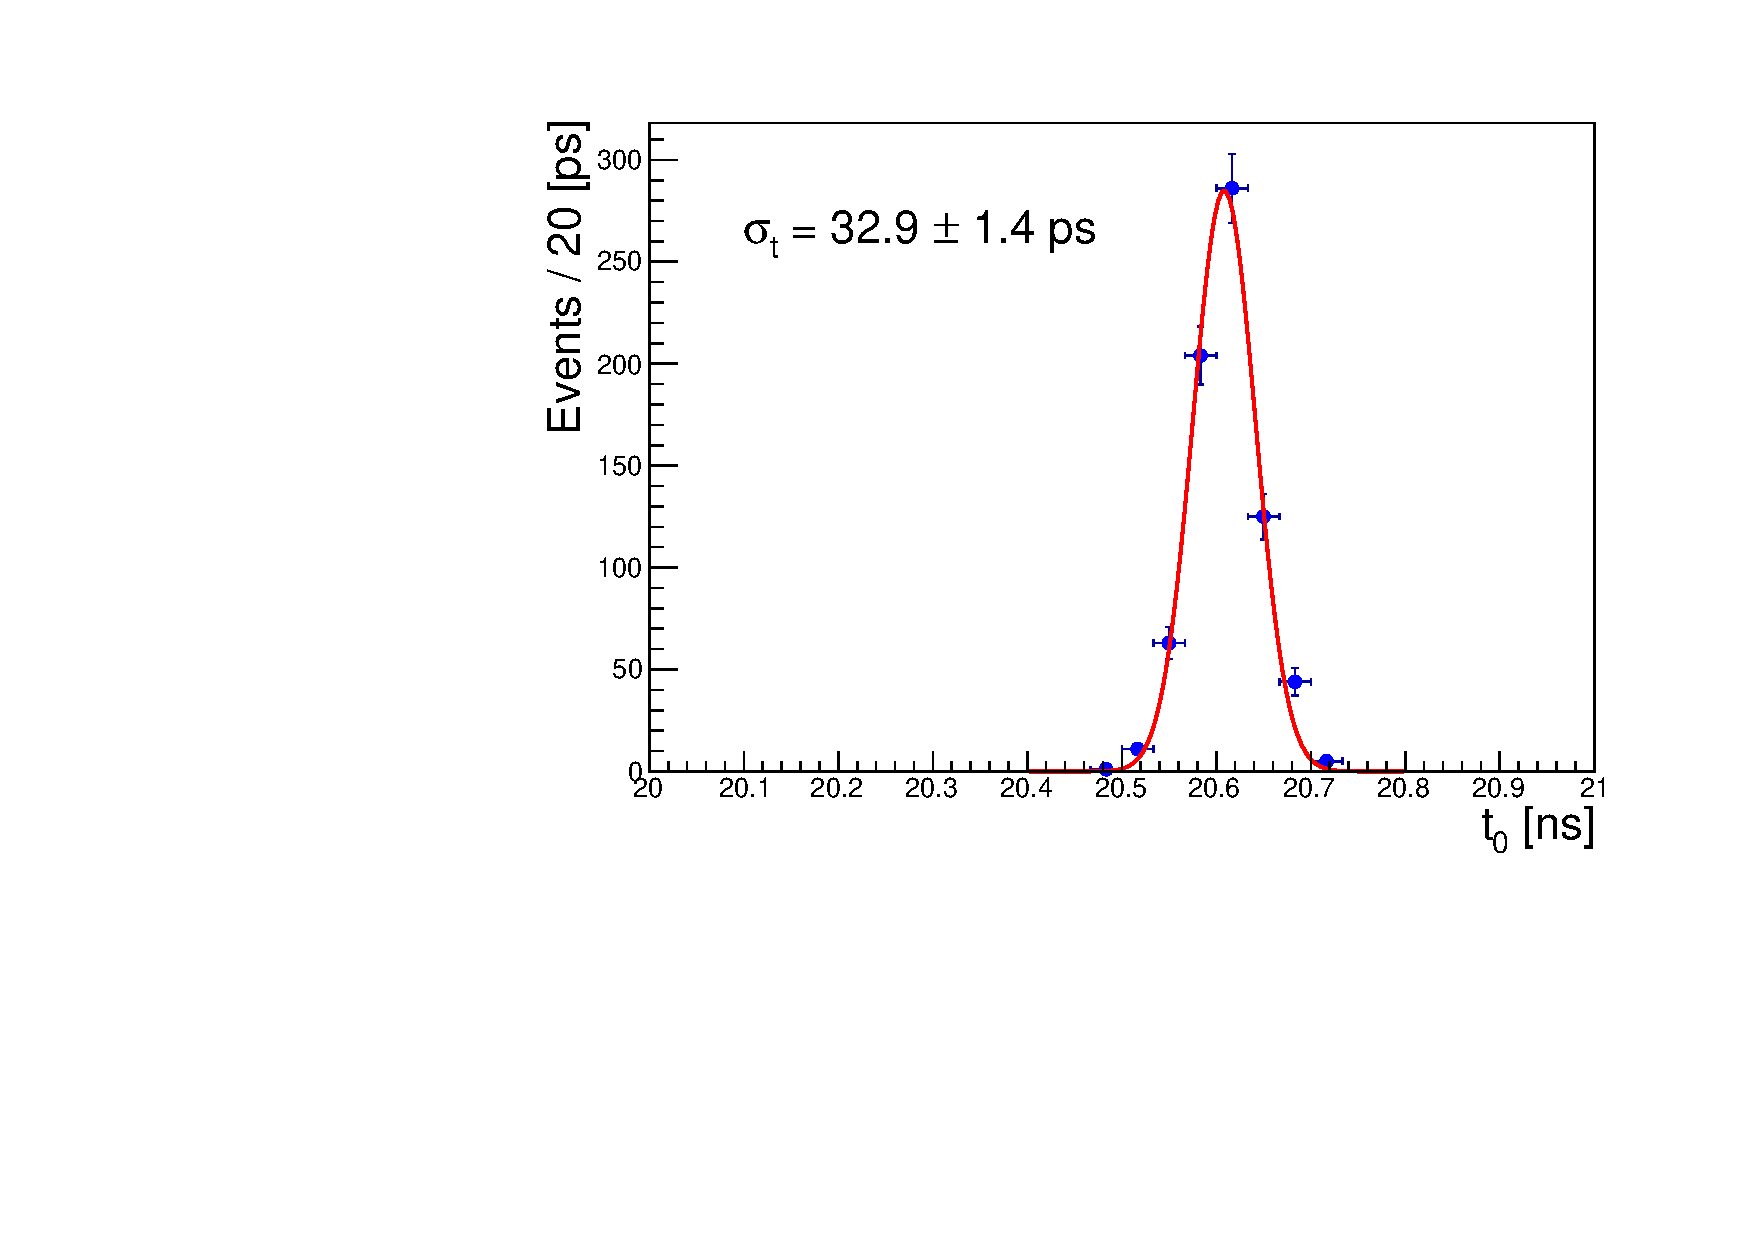
\includegraphics[width=0.48\textwidth]{figs/pre_rad_st_1ns_snr_30_cfd_tot_threshold_35_percent_v2.pdf}
    \caption{(Left) timestamp ($t_{0}$) distribution for a 30~\si{mV} threshold using a leading edge discriminator.
    (Right) timestamp ($t_{0}$) distribution for a 35\% threshold using a constant fraction discriminator. Both figures
    include the time-walk correction based on the measured ToT.
    Both figures use pre-radiated unprocessed pulses, a shaping time (ST) of 1~\si{ns}, and correspond to SNR of 30.}
    \label{fig:time_res}
  \end{figure}
  
  

\section{LGAD front-end electronics performance}\label{sec:results}

We discuss first studies of the FEE performance as a function of the shaping time and SNR.
The results for the pre-irradiated LGAD sensor are summarized in Table~\ref{tab:prerad},
where the CF results are from the ideal implementation.  Table~\ref{tab:prerad_psCFD}
shows the time resolution results for the practical CF implementation using the RC-type low pass filter,
where we observe a degradation in performance, which grows as the SNR decreases.

We observe that the best results are consistently obtained for ST of 0.5~\si{ns} and 1.0~\si{ns} STs regardless of the SNR. 
We observe that larger STs are more affected by less favorable SNR. For example, for an SNR of 20, the time resolution is ~37~\si{ps} and ~100~\si{ps} for a ST of 0.5~\si{ns} and 4.0~\si{ns}, respectively. We note that CF consistently outperforms 
LE, and this effect is also observed for less favorable SNR and slower ST. Comparing CF and LE for the 1.0~\si{ns} ST 
with SNR of 20 yields a difference in performance of 26~\si{ps}, when subtracted in quadrature. In summary, for 
pre-irradiated sensors we observed that time resolutions of ~35~\si{ps} are achievable for
STs between 0.5 - 1.0~\si{ns} and a SNR of 30.

\begin{table}
    \begin{tabular}{c|ccc|ccc}
    \multicolumn{1}{c}{}& \multicolumn{6}{c}{Time Resolution (ps)} \\
    \multicolumn{1}{c}{}&\multicolumn{3}{c}{Leading Edge} & \multicolumn{3}{c}{Constant Fraction (Ideal)}\\ \hline
    ST (ns) & SNR = 20   & SNR = 30      & SNR = 100     & SNR = 20      & SNR = 30      & SNR = 100 \\
    0.5 & $38$    & $35$  & $29$  & $37$  & $35$  & $30$ \\
    1.0 & $45$    & $37$  & $29$  & $36$  & $33$  & $26$ \\
    2.0 & $63$    & $48$  & $31$  & $48$  & $34$  & $29$ \\
    4.0 & $103$  & $75$  & $38$  & $74$  & $55$  & $32$ \\
    \end{tabular}
    \caption{50~$\mu$m pre-radiation LGAD sensor simulation: summary of best time resolution obtained for SNRs
    of 20, 30, and 100. Leading edge and constant fraction results are shown. The measured time resolutions
    have statistical uncertainty below 5\%. }
    \label{tab:prerad}
 \end{table}


 \begin{table}
   \begin{center}
     \begin{tabular}{c|ccc}
     \multicolumn{1}{c}{}& \multicolumn{3}{c}{Time Resolution (ps)} \\
     \multicolumn{1}{c}{}& \multicolumn{3}{c}{$\mathrm{(RC)}^{2}$ Constant Fraction}\\ \hline
     ST (ns) & SNR = 20      & SNR = 30      & SNR = 100 \\
     1.0 & $58$  & $ 40$  & $28$ \\
     2.0 & $68$  & $ 49$  & $30$ \\     
     \end{tabular}
     \caption{50~$\mu$m pre-radiation LGAD sensor using a second order RC implementation of a CFD.
     Summary of best time resolution obtained using a ST of 2\si{ns} for SNRs of 20, 30, and 100. The measured time resolutions
    have statistical uncertainty below 5\%.}
     \label{tab:prerad_psCFD}
   \end{center}
  \end{table}


We study the effect of irradiation on the time resolution of a 50~$\mu$m LGAD sensor. The impact of irradiation on the unprocessed signal pulse shapes are simulated for by the WF2 simulation. The width of the unprocessed
LGAD signal pulses decrease slightly as the irradiation dosage increases. We consider two
cases with neutron fluences of $5\times 10^{14}$~n/cm$^2$ and 
$1\times 10^{15}$~n/cm$^2$. We perform the same studies as in the pre-irradiated case. 
The results for the irradiated LGAD sensors are presented in 
Tables~\ref{tab:shaping_time_5e14}~and~\ref{tab:shaping_time_5e14_psCFD} for 
neutron fluences of $5\times 10^{14}$~n/cm$^2$, and in 
Tables~\ref{tab:shaping_time_1e_15}~and~\ref{tab:shaping_time_1e15_psCFD} for neutron
fluences of $1\times 10^{15}$~n/cm$^2$.
We observe similar trends as observed for the pre-irradiated sensor and note that when 
using STs between 0.5 - 1.0~\si{ns} and a SNR of 30, time resolutions of the order
of 31~\si{ps}~and~37~\si{ps} are obtained for $5\times 10^{14}$~n/cm$^2$ and 
$1\times 10^{15}$~n/cm$^2$, respectively.





 \begin{table}
     \begin{tabular}{c|ccc|ccc}
     \multicolumn{1}{c}{}& \multicolumn{6}{c}{Time Resolution (ps)} \\
     \multicolumn{1}{c}{}&\multicolumn{3}{c}{Leading Edge} & \multicolumn{3}{c}{Constant Franction}\\ \hline
     ST (ns) & SNR = 20   & SNR = 30      & SNR = 100     & SNR = 20      & SNR = 30      & SNR = 100 \\
     0.5 & $37$  & $32$  & $26$  & $33$  & $31$  & $25$ \\
     1.0 & $41$  & $34$  & $29$  & $33$  & $31$  & $26$ \\
     2.0 & $57$  & $45$  & $30$  & $44$  & $37$  & $24$ \\
     4.0 & $93$  & $68$  & $37$  & $71$  & $52$  & $30$ \\
     \end{tabular}
     \caption{50~$\mu$m LGAD sensor simulation after neutron fluence of
      $5\times 10^{14}$~n/cm$^2$: summary of best time resolution obtained for SNRs
     of 20, 30, and 100. Leading edge and constant fraction results are shown. The measured time resolutions
    have statistical uncertainty below 5\%.}
\label{tab:shaping_time_5e14}
  \end{table}

 \begin{table}
    \begin{center}
     \begin{tabular}{c|ccc|ccc}
     \multicolumn{1}{c}{}& \multicolumn{3}{c}{Time Resolution (ps)} \\
     \multicolumn{1}{c}{}& \multicolumn{3}{c}{$\mathrm{(RC)}^{2}$ Constant Fraction}\\ \hline
     ST (ns) & SNR = 20      & SNR = 30      & SNR = 100 \\
     1.0 & $55$  & $ 37$  & $30$ \\
     2.0 & $70$  & $ 53$  & $33$ \\     
     \end{tabular}
     \end{center}
     \caption{50~$\mu$m LGAD sensor simulation after neutron fluence of
      $5\times 10^{14}$~n/cm$^2$ using a second order RC implementation of a CFD. 
      Summary of best time resolution obtained for SNRs
     of 20, 30, and 100. The measured time resolutions
    have statistical uncertainty below 5\%.}
\label{tab:shaping_time_5e14_psCFD}
  \end{table}




  \begin{table}
      \begin{tabular}{c|ccc|ccc}
      \multicolumn{1}{c}{}& \multicolumn{6}{c}{Time Resolution (ps)} \\
      \multicolumn{1}{c}{}&\multicolumn{3}{c}{Leading Edge} & \multicolumn{3}{c}{Constant Franction}\\ \hline
      ST (ns) & SNR = 20   & SNR = 30      & SNR = 100     & SNR = 20      & SNR = 30      & SNR = 100 \\
      0.5 & $48$    & $38$    & $27$  & $42$    & $34$  & $24$ \\
      1.0 & $60$    & $47$    & $28$  & $47$    & $37$  & $23$ \\
      2.0 & $90$    & $68$    & $32$  & $65$    & $50$  & $27$ \\
      4.0 & $147$  & $109$  & $43$  & $119$  & $84$  & $34$ \\
      \end{tabular}
      \caption{50~$\mu$m LGAD sensor simulation after neutron fluence of
       $1\times 10^{15}$~n/cm$^2$: Summary of best time resolution obtained for SNRs
      of 20, 30, and 100. Leading edge and constant fraction results are shown. The measured time resolutions
    have statistical uncertainty below 5\%.}
\label{tab:shaping_time_1e_15}
   \end{table}


 \begin{table}
    \begin{center}
     \begin{tabular}{c|ccc|ccc}
     \multicolumn{1}{c}{}& \multicolumn{3}{c}{Time Resolution (ps)} \\
     \multicolumn{1}{c}{}& \multicolumn{3}{c}{$\mathrm{(RC)}^{2}$ Constant Fraction}\\ \hline
     ST (ns) & SNR = 20      & SNR = 30      & SNR = 100 \\
     1.0 & $45$  & $ 39$  & $29$ \\
     2.0 & $83$  & $ 53$  & $33$ \\     
     \end{tabular}
     \end{center}
     \caption{50~$\mu$m LGAD sensor simulation after neutron fluence of
      $1\times 10^{15}$~n/cm$^2$ using a second order RC implementation of a CFD. 
      Summary of best time resolution obtained for SNRs
     of 20, 30, and 100. The measured time resolutions
    have statistical uncertainty below 5\%. }
\label{tab:shaping_time_1e15_psCFD}
  \end{table}
  
  
\section{Conclusion}\label{sec:conclusion}

We study the time resolution of a 50~$\mu$m Low-gain avalanche diode (LGAD) 
sensor using a simulation framework that includes the
modeling of raw LGAD signal pulses, the front-end readout electronics (FEE), and effects of 
time-to-digital converter quantization resolution.
Using a second order low-pass filter to model the FEE, 
we focused on studying the impact of the shaping time (ST) and signal-to-noise ratio (SNR) of the FEE 
on the time resolution performance, as well as its dependence on the irradiation level of the sensor. 
We observe a clear degradation of the time resolution with SNR and slower STs. The best results are
obtained using a ST of 0.5~\si{ns} and using constant fraction (CF) discriminator, and similar 
results are obtained with a ST of 1.0~\si{ns}. For a SNR of 30 and for STs between 0.5-1.0~\si{ns} we 
obtain time resolutions between ~30 - 37~\si{ps} for the range of sensor irradiation relevant for the MIP timing detectors
proposed for the HL-LHC. The reduction in gain with irradiation could bring the SNR for the most irradiated 
LGAD ($1\times 10^{15}$~n/cm$^2$) to 20 and thus worsen the time resolution to ~42 - 47~\si{ps}. 
We note a clear gain in performance of CF over leading edge (LE) discriminators, particularly at
low SNR and the largest irradiation level. For an ST of 1.0~\si{ns} at SNR = 30, the performance improvement of 
CF over LE is ~26\si{ps} for the pre-irradiated sensor and ~37\si{ps} for the irradiated sensor with neutron fluence of
$1\times 10^{15}$~n/cm$^2$. A small performance degradation is observed when using a more
realistic implementation of the CFD, especially at lower SNRs. Overall our simulation results indicate that 
time resolutions better than 45~\si{ps} are achievable for a 50~$\mu$m LGADs for irradiation levels up 
to neutron fluences of $1\times 10^{15}$~n/cm$^2$.


\section*{Acknowledgment}

The authors will like to thank N. Cartiglia, T. Liu, and S. Los for insightful discussions.

A. Apresyan gratefully acknowledges support from the DOE Early Career Research Program.
This document was prepared using the resources of the Fermi National Accelerator
Laboratory (Fermilab), a U.S. Department of Energy, Office of Science, HEP User
Facility. Fermilab is managed by Fermi Research Alliance, LLC (FRA), acting
under Contract No. DE-AC02-07CH11359. Part of this work was performed within the
framework of the CERN RD50 collaboration.

This work was supported by the Fermilab LDRD 2017.027; by the U.S.
Department of Energy grant DE-FG02-04ER41286; by the California Institute of
Technology High Energy Physics grant from the U.S.
Department of Energy under Contract DE-SC0011925; by the European
Union's Horizon 2020 Research and Innovation funding program, under Grant
Agreement no. 654168 (AIDA-2020) and Grant Agreement no. 669529 (ERC
UFSD669529); by the Italian Ministero degli Affari Esteri and INFN Gruppo V; and
by the Spanish Ministry of Economy, Industry and Competitiveness through the
Particle Physics National Program (ref. FPA2014-55295-C3-2-R and
FPA2015-69260-C3-3-R) co-financed with FEDER funds.

% The Appendices part is started with the command \appendix;
% appendix sections are then done as normal sections

%\appendix
%\section{Appendix A}



% \section{}
% \label{}

%% If you have bibdatabase file and want bibtex to generate the
%% bibitems, please use
%%
%%  \bibliographystyle{elsarticle-num}
%%  \bibliography{<your bibdatabase>}

%% else use the following coding to input the bibitems directly in the
%% TeX file.

\bibliography{lgad_frontend_simulation}{}
\bibliographystyle{ieeetr}

%\begin{thebibliography}{00}

%% \bibitem{label}
%% Text of bibliographic item

%\bibitem{}

%\end{thebibliography}
\end{document}
\endinput
%%
%% End of file `elsarticle-template-num.tex'.
